% Options for packages loaded elsewhere
% Options for packages loaded elsewhere
\PassOptionsToPackage{unicode}{hyperref}
\PassOptionsToPackage{hyphens}{url}
\PassOptionsToPackage{dvipsnames,svgnames,x11names}{xcolor}
%
\documentclass[
  letterpaper,
  DIV=11,
  numbers=noendperiod]{scrartcl}
\usepackage{xcolor}
\usepackage[margin=1in]{geometry}
\usepackage{amsmath,amssymb}
\setcounter{secnumdepth}{5}
\usepackage{iftex}
\ifPDFTeX
  \usepackage[T1]{fontenc}
  \usepackage[utf8]{inputenc}
  \usepackage{textcomp} % provide euro and other symbols
\else % if luatex or xetex
  \usepackage{unicode-math} % this also loads fontspec
  \defaultfontfeatures{Scale=MatchLowercase}
  \defaultfontfeatures[\rmfamily]{Ligatures=TeX,Scale=1}
\fi
\usepackage{lmodern}
\ifPDFTeX\else
  % xetex/luatex font selection
  \setmainfont[]{Times New Roman}
\fi
% Use upquote if available, for straight quotes in verbatim environments
\IfFileExists{upquote.sty}{\usepackage{upquote}}{}
\IfFileExists{microtype.sty}{% use microtype if available
  \usepackage[]{microtype}
  \UseMicrotypeSet[protrusion]{basicmath} % disable protrusion for tt fonts
}{}
\makeatletter
\@ifundefined{KOMAClassName}{% if non-KOMA class
  \IfFileExists{parskip.sty}{%
    \usepackage{parskip}
  }{% else
    \setlength{\parindent}{0pt}
    \setlength{\parskip}{6pt plus 2pt minus 1pt}}
}{% if KOMA class
  \KOMAoptions{parskip=half}}
\makeatother
% Make \paragraph and \subparagraph free-standing
\makeatletter
\ifx\paragraph\undefined\else
  \let\oldparagraph\paragraph
  \renewcommand{\paragraph}{
    \@ifstar
      \xxxParagraphStar
      \xxxParagraphNoStar
  }
  \newcommand{\xxxParagraphStar}[1]{\oldparagraph*{#1}\mbox{}}
  \newcommand{\xxxParagraphNoStar}[1]{\oldparagraph{#1}\mbox{}}
\fi
\ifx\subparagraph\undefined\else
  \let\oldsubparagraph\subparagraph
  \renewcommand{\subparagraph}{
    \@ifstar
      \xxxSubParagraphStar
      \xxxSubParagraphNoStar
  }
  \newcommand{\xxxSubParagraphStar}[1]{\oldsubparagraph*{#1}\mbox{}}
  \newcommand{\xxxSubParagraphNoStar}[1]{\oldsubparagraph{#1}\mbox{}}
\fi
\makeatother


\usepackage{longtable,booktabs,array}
\newcounter{none} % for unnumbered tables
\usepackage{calc} % for calculating minipage widths
% Correct order of tables after \paragraph or \subparagraph
\usepackage{etoolbox}
\makeatletter
\patchcmd\longtable{\par}{\if@noskipsec\mbox{}\fi\par}{}{}
\makeatother
% Allow footnotes in longtable head/foot
\IfFileExists{footnotehyper.sty}{\usepackage{footnotehyper}}{\usepackage{footnote}}
\makesavenoteenv{longtable}
\usepackage{graphicx}
\makeatletter
\newsavebox\pandoc@box
\newcommand*\pandocbounded[1]{% scales image to fit in text height/width
  \sbox\pandoc@box{#1}%
  \Gscale@div\@tempa{\textheight}{\dimexpr\ht\pandoc@box+\dp\pandoc@box\relax}%
  \Gscale@div\@tempb{\linewidth}{\wd\pandoc@box}%
  \ifdim\@tempb\p@<\@tempa\p@\let\@tempa\@tempb\fi% select the smaller of both
  \ifdim\@tempa\p@<\p@\scalebox{\@tempa}{\usebox\pandoc@box}%
  \else\usebox{\pandoc@box}%
  \fi%
}
% Set default figure placement to htbp
\def\fps@figure{htbp}
\makeatother


% definitions for citeproc citations
\NewDocumentCommand\citeproctext{}{}
\NewDocumentCommand\citeproc{mm}{%
  \begingroup\def\citeproctext{#2}\cite{#1}\endgroup}
\makeatletter
 % allow citations to break across lines
 \let\@cite@ofmt\@firstofone
 % avoid brackets around text for \cite:
 \def\@biblabel#1{}
 \def\@cite#1#2{{#1\if@tempswa , #2\fi}}
\makeatother
\newlength{\cslhangindent}
\setlength{\cslhangindent}{1.5em}
\newlength{\csllabelwidth}
\setlength{\csllabelwidth}{3em}
\newenvironment{CSLReferences}[2] % #1 hanging-indent, #2 entry-spacing
 {\begin{list}{}{%
  \setlength{\itemindent}{0pt}
  \setlength{\leftmargin}{0pt}
  \setlength{\parsep}{0pt}
  % turn on hanging indent if param 1 is 1
  \ifodd #1
   \setlength{\leftmargin}{\cslhangindent}
   \setlength{\itemindent}{-1\cslhangindent}
  \fi
  % set entry spacing
  \setlength{\itemsep}{#2\baselineskip}}}
 {\end{list}}
\usepackage{calc}
\newcommand{\CSLBlock}[1]{\hfill\break\parbox[t]{\linewidth}{\strut\ignorespaces#1\strut}}
\newcommand{\CSLLeftMargin}[1]{\parbox[t]{\csllabelwidth}{\strut#1\strut}}
\newcommand{\CSLRightInline}[1]{\parbox[t]{\linewidth - \csllabelwidth}{\strut#1\strut}}
\newcommand{\CSLIndent}[1]{\hspace{\cslhangindent}#1}



\setlength{\emergencystretch}{3em} % prevent overfull lines

\providecommand{\tightlist}{%
  \setlength{\itemsep}{0pt}\setlength{\parskip}{0pt}}



 


\usepackage{booktabs}
\usepackage{caption}
\usepackage{longtable}
\usepackage{colortbl}
\usepackage{array}
\usepackage{anyfontsize}
\usepackage{multirow}
\KOMAoption{captions}{tableheading}
\usepackage{longtable}
\usepackage{booktabs}
\usepackage{setspace}
\doublespacing
\documentclass[12pt,a4paper]{article}
\usepackage{caption}
\usepackage{fancyhdr}
\pagestyle{fancy}
\fancyhf{}
\rfoot{Page \thepage}
\usepackage[bottom]{footmisc}
\usepackage{hyperref}
\hypersetup{colorlinks=true, linkcolor=black, urlcolor=black, citecolor=black, allcolors=black}
\AtBeginDocument{\hypersetup{hidelinks}}
\makeatletter
\@ifpackageloaded{caption}{}{\usepackage{caption}}
\AtBeginDocument{%
\ifdefined\contentsname
  \renewcommand*\contentsname{Table of contents}
\else
  \newcommand\contentsname{Table of contents}
\fi
\ifdefined\listfigurename
  \renewcommand*\listfigurename{List of Figures}
\else
  \newcommand\listfigurename{List of Figures}
\fi
\ifdefined\listtablename
  \renewcommand*\listtablename{List of Tables}
\else
  \newcommand\listtablename{List of Tables}
\fi
\ifdefined\figurename
  \renewcommand*\figurename{Figure}
\else
  \newcommand\figurename{Figure}
\fi
\ifdefined\tablename
  \renewcommand*\tablename{Table}
\else
  \newcommand\tablename{Table}
\fi
}
\@ifpackageloaded{float}{}{\usepackage{float}}
\floatstyle{ruled}
\@ifundefined{c@chapter}{\newfloat{codelisting}{h}{lop}}{\newfloat{codelisting}{h}{lop}[chapter]}
\floatname{codelisting}{Listing}
\newcommand*\listoflistings{\listof{codelisting}{List of Listings}}
\makeatother
\makeatletter
\makeatother
\makeatletter
\@ifpackageloaded{caption}{}{\usepackage{caption}}
\@ifpackageloaded{subcaption}{}{\usepackage{subcaption}}
\makeatother
\usepackage{bookmark}
\IfFileExists{xurl.sty}{\usepackage{xurl}}{} % add URL line breaks if available
\urlstyle{same}
\hypersetup{
  colorlinks=true,
  linkcolor={blue},
  filecolor={Maroon},
  citecolor={Blue},
  urlcolor={Blue},
  pdfcreator={LaTeX via pandoc}}


\author{}
\date{}
\begin{document}


\begin{titlepage}
\centering

\vspace*{2cm}

{\Huge Beyond the One-Hour Standard: Using Auxiliary Data to Reconstruct Nigeria's Discontinued Unemployment Series \par}

\vspace{2cm}

by

\vspace{1cm}

{\Large 72601\par}

\vspace{1cm}

A Capstone Project submitted in partial fulfilment
of the requirements for the degree of
MSc Applied Social Data Science

\vspace{1cm}

at

\vfill

Department of Methodology\\
London School of Economics and Political Science\\

\vspace{1cm}

Supervisor: Tom Robinson

July 2026

Estimated Word Count: 9913

\end{titlepage}
\newpage

\textbf{Abstract}

The adoption of the International Labour Organization (ILO) definition
of unemployment and the consequent discontinuation of domestic measures
in many developing countries have attracted substantial criticism,
particularly around its limited representation of local labour-market
conditions. While there have been theoretical debates on the utility of
domestic definitions, few empirical studies have attempted to
reconstruct them once they are officially discontinued.

This study addresses that gap by examining Nigeria's recent adoption of
the ILO definition. Using machine-learning techniques, it seeks to
reconstruct the discontinued domestic unemployment measure from
available long-term data series. The research is motivated by the
drastic change in reported unemployment rates following the adoption of
the new definition.

To achieve this objective, the study compiles administrative and
alternative data sources to estimate the previous measure of
unemployment. It additionally compares the determinants of both
definitions using model coefficients to assess whether their differences
extend beyond the effect of arbitrary threshold changes. An elastic net
model is adopted as the most appropriate modelling framework within the
Nigeria context, specifically, for its unique feature selection and
extrapolation abilities. The findings suggest that the previous
unemployment definition can be reconstructed with reasonable accuracy
for the years examined. However, validation for future periods is not
possible because the measure has been discontinued.

More importantly, the results indicate that although both definitions
share several common drivers, certain socioeconomic factors influence
them differently. These differences suggest that changes in
classification thresholds create structurally distinct unemployment
metrics.

\clearpage

\newpage

\tableofcontents

\listoffigures

\listoftables

\newpage

\section{Introduction}\label{introduction}

\subsection{Background and Motivation}\label{background-and-motivation}

Since 1923, the International Conference of Labour Statisticians (ICLS),
a technical body of the International Labour Organization (ILO), has
worked to develop international guidelines that standardize how
countries define concepts related to work, employment, and labour
statistics \footnote{Table~\ref{tbl-icls-sessions}}. While the
conference has produced standards adopted widely across countries, the
structural diversity of economies around the world often generates
debates on their applicability (Brandolini et al. 2006; Guataquí and
Taborda 2006; Baah-Boateng 2015; Alenda-Demoutiez and Mügge 2020). A
clear illustration of these structural differences can be seen in
Table~\ref{tbl-country_minwage}, which shows the varying units of works
countries use to define their minimum wages --- some fixing an hourly
rate, others a monthly rate, and some formally recognizing both. This
variation is not merely administrative; since the ILO defines employment
as work performed for pay or profit, differences in how pay is
standardized across countries raise the recurring question of whether a
single unemployment standard can be applied uniformly across such
diverse labour economies.

Notably, there are persistent concerns regarding the applicability of
international labour standards in developing economies characterized by
high levels of informality, where the consequences of statistical
mismeasurement are particularly severe (Byrne and Strobl 2004;
Alenda-Demoutiez and Mügge 2020). Scholars and practitioners have
extensively debated several core tenets of the standard employment
definition to determine their validity in developing contexts. Key
contentions include whether an ``active job search'' should be strictly
required to classify an individual as unemployed, and whether the
minimum working-hour thresholds accurately reflect labour market
realities (Brandolini et al. 2006; Hussmanns 2007; Byrne and Strobl
2004). The validity of these debates have been acknowledge by the ILO
and broader, composite measures of labour underutilization (LU1--LU4)
have sprang up in recent years (International Labour Organization 2011;
International Conference of Labour Statisticians 2023).

The differences in measures resulting from different definitions are
significant to policy and national decision making. Nigeria's National
Bureau of Statistics (NBS) provides a contemporary case study where this
can be explored, having maintained a domestically adapted unemployment
definition for over two decade before fully transitioning to the ILO
standard in 2023 (National Bureau of Statistics 2023; World Bank, n.d.).
Prior to this methodological shift, Nigeria's NBS operated under a
framework that initially classified individuals working less than 40
hours a week as unemployed (Kale and Doguwa 2015), a threshold that was
later revised downward to 20 hours per week (National Bureau of
Statistics 2021; Kale and Doguwa 2015). Under this stringent domestic
framework, Nigeria recorded a headline unemployment rate of 33.3\% in
the fourth quarter of 2020 (World Bank, n.d.; National Bureau of
Statistics 2021).

Following the transition to the ILO definition, which classifies
individuals as employed if they worked for at least one hour for pay or
profit during the reference week, the reported unemployment rate
plummeted to 5.3\% in the fourth quarter of 2022 (World Bank, n.d.;
National Bureau of Statistics 2023). This drastic statistical decline
was driven almost entirely by the definitional and methodological shift,
rather than a substantive improvement in underlying labour market
conditions during the intervening period.

Consequently, several stakeholders have publicly criticized the change
of methodology and others have outrightly dismissed the new figures
(Proshare Research 2023; Aro 2023; Daily Trust 2023). This is consistent
with arguements in literature stating that domestically adapted
methodologies are arguably better suited to the economic reality of
developing labour markets, where informal subsistence work and chronic
underemployment are pervasive (Baah-Boateng 2015; World Bank, n.d.).

Despite the widespread recognition that labour market fluctuations are
intricately linked to structural macroeconomic indicators and
non-traditional data source (Askitas and Zimmermann 2009; Choi 2009)
that continues to be available, there has been no empirical attempt to
systematically reconstruct the discontinued, domestically adapted
employment series to preserve historical continuity.

\subsection{Research Question and
Scope}\label{research-question-and-scope}

The 2023 adoption of the ILO's one-hour employment criterion marked a
major break in Nigeria's labour statistics. While the transition
improved alignment with international standards, it also resulted in the
discontinuation of the unemployment series previously produced under
Nigeria's domestic methodology. Consequently, researchers, policymakers,
and the public can no longer directly compare contemporary unemployment
figures with historical estimates constructed using the earlier
framework.

This discontinuity creates two important challenges. First, it limits
the ability to assess changes in labour market conditions over time
because observed differences in unemployment rates may reflect
methodological changes rather than genuine economic developments.
Second, it raises broader questions regarding the suitability of
international labour standards in economies characterised by high levels
of informality and underemployment.

This study addresses these challenges by investigating whether auxiliary
data sources can be used to reconstruct Nigeria's discontinued
unemployment series. In particular, it examines whether administrative
indicators and digital trace data can recover the variation previously
captured by Nigeria's domestic unemployment definition.

The primary research question is:

\emph{To what extent can auxiliary socioeconomic indicators and digital
trace data accurately reconstruct Nigeria's discontinued unemployment
series?}

To answer this question, the study considers three subsidiary questions:

Which socioeconomic and/or digital trace indicators are most predictive
of unemployment under Nigeria's discontinued domestic definition?

What modelling framework can be used to learn the discontinued domestic
unemployment definition?

How accurately can the machine learning model reconstruct historical
unemployment rates using these indicators?

The study focuses on the period for which both unemployment statistics
and auxiliary indicators are available, combining administrative
macroeconomic data with digital search data. Rather than creating a new
independent index for unemployment, the objective of this study is to
assess whether discontinued unemployment rate series can be
reconstructed in a statistically reliable manner and to explore what
such reconstruction reveals about labour market distress in a
high-informality economy.

By doing so, the study contributes to both the methodological literature
on reconstructing discontinued statistical series and the broader debate
regarding the measurement of unemployment in developing economies.

\subsection{Contributions}\label{contributions}

This study contributes to the literature in four ways. First, it
develops a framework for reconstructing labour market indicators
following major methodological breaks in official statistics. While
changes in statistical definitions are common, relatively little
attention has been paid to how discontinued series can be systematically
recovered to preserve historical continuity and enable longitudinal
analysis. By combining macroeconomic indicators with recursive
forecasting techniques, this study demonstrates a practical approach for
extending discontinued labour market series beyond their official
publication period.

Second, the study contributes new empirical evidence from a highly
informal labour market context. Most unemployment nowcasting and
reconstruction studies have been conducted in advanced economies
characterized by formal labour markets and relatively stable statistical
definitions. Nigeria provides a substantially different environment,
where labour market participation is dominated by informal and
survival-oriented activities, making it an important case for evaluating
the robustness of reconstruction approaches.

Third, the study provides a direct comparison of the macroeconomic
determinants associated with alternative unemployment definitions.
Rather than treating unemployment as a fixed statistical construct, the
analysis recognizes that different definitions capture different
dimensions of labour market distress. Comparing the historical Nigerian
definition with the ILO framework allows the study to examine whether
different methodological definitions respond similarly to the broader
economic conditions.

Finally, the study contributes to broader debates concerning statistical
harmonization in developing economies. While internationally
standardized indicators facilitate cross-country comparison, they may
also obscure locally relevant dimensions of economic hardship. The
findings therefore speak not only to unemployment measurement in Nigeria
but also to wider questions concerning the balance between international
comparability and domestic policy relevance in official statistics.

The remainder of this paper is structured as follows: Section 2 reviews
the relevant literature, Section 3 describes the data and methodology,
Section 4 presents the results, and Section 5 discusses the findings and
concludes.

\section{Literature Review}\label{literature-review}

This section reviews the difficulties around operationalizing
unemployment in developing countries alongside academic literature on
the reconstruction and estimation of labour market indicators in
contexts of sparse or incomplete data. It is structured in three main
parts. First, it discusses debates on the adaptation of ILO standards in
developing countries. Second, it reviews Nigeria as a contextual case
study. Finally, it examines likely data sources and methodological
frameworks to estimate unemployment rates.

\subsection{Measuring Unemployment in Developing
Economies}\label{measuring-unemployment-in-developing-economies}

The conceptualization and measurement of unemployment have been subjects
of intense historical and methodological debate. The earliest efforts to
establish international statistical standards for unemployment trace
back to 1895, when the International Statistical Institute in Berne
attempted to address the non-comparability of unemployment statistics
across industrialised European nations (Richardson et al. 1992). Through
successive International Conferences of Labour Statisticians (ICLS)
shown in Table~\ref{tbl-icls-sessions}, particularly the Eighth ICLS in
1954, the modern labour force framework was established. This framework
officially defined the unemployed as individuals of working age who are
simultaneously ``without work,'' ``currently available for work,'' and
``actively seeking work'' (Byrne and Strobl 2004; Richardson et al.
1992).

However, the strict application of these criteria generated persistent
theoretical contention, leading scholars and national statisticians to
question their validity in developing economies (Byrne and Strobl 2004).
Historically, the statistical category of unemployment was constructed
to measure labour distress in advanced, industrialized nations where
formal wage-labour is the dominant social norm and where safety nets,
such as unemployment insurance, allow individuals to visibly engage in
active job searching (Benanav 2019; International Labour Organization
2011). In Low-Income Developing Countries (LIDCs), these structural
conditions are fundamentally absent (Benanav 2019) as formal labour
exchange channels are limited and comprehensive unemployment benefits
are practically non-existent, the vast majority of the population cannot
afford to remain completely idle (Baah-Boateng 2015; Morse 1970).
Consequently, when formal jobs are scarce, workers are forced to take up
low-productivity, informal survival activities or subsistence
agriculture (Benanav 2019; Baah-Boateng 2015).

These structural realities have caused researchers and national
statistical agencies to conclude that implementing domestically adapted
definitions is not merely a deviation from international norms, but a
statistically valid and necessary requirement for capturing true
economic distress. As strictly applying the ILO's standard criteria in
LIDCs can artificially deflate the unemployment rate, creating an
``unemployment-informality trade-off'' where high levels of precarious
employment actively conceal true joblessness (Baah-Boateng 2015).

Several nations have historically adopted broad, domestic adaptations of
unemployment definitions to correct these biases (Alenda-Demoutiez and
Mügge 2020; Guataquí and Taborda 2006). For example, in early
post-Apartheid South Africa, statisticians consciously defied
international conventions to utilize an expanded unemployment indicator;
this domestic adaptation was institutionally validated because it
corrected the severe gendered and racialized biases of the strict ILO
definition, thereby doing justice to the discouraged, marginalized Black
population (Alenda-Demoutiez and Mügge 2020). Similarly, Trinidad and
Tobago officially dropped the active job search requirement from its
national definition, an adaptation empirically validated by research
demonstrating that non-searching, marginally attached workers in
developing nations possess the same transitional labour market behaviour
as active job seekers (Guataquí and Taborda 2006; Byrne and Strobl
2004).

The theoretical validity of these domestic adaptations was ultimately
recognized by the ILO itself. Acknowledging that the standard
unemployment definition could be overly restrictive in certain labour
market contexts, the 13th International Conference of Labour
Statisticians (ICLS) in 1982 introduced a ``relaxation provision''
(Hussmanns 2007; Richardson et al. 1992). This provision explicitly
permitted countries to relax the ``seeking work'' criterion in
situations where labour markets were largely unorganized, where
conventional job-search mechanisms were of limited relevance, or where
self-employment constituted the dominant form of economic activity
(International Labour Organization 1982; Richardson et al. 1992).

The ILO additionally addressed these limitations by argumenting the base
unemployment measure and introducing several other labour untilization
measures to help developing contexts characterized by widespread
informality, precarious work, and underemployment (International Labour
Organization 2011). These formal altercations and adjustments lend
credibility to the need to having different unemployment definitions for
less developing economies.

Despite this institutional flexibility and the acknowledgement that
labour market realities differ substantially across countries, the
political economy of global statistics --- driven by international
financial institutions, donor agencies, and the pursuit of cross-country
comparability --- has often encouraged developing nations to align with
standardized international definitions. As a result, domestically
adapted measures are sometimes abandoned in favour of harmonized
indicators, even when local statisticians argue that such adaptations
better reflect national labour market conditions (Alenda-Demoutiez and
Mügge 2020).

\subsection{Nigeria's Labour Market and Statistical
Transition}\label{nigerias-labour-market-and-statistical-transition}

Nigeria was historically one of the countries that actively developed a
domestic adaptation of the unemployment definition and regularly
reviewed it against the realities of its labour market (Kale and Doguwa
2015). In keeping with its statutory mandate, the National Bureau of
Statistics (NBS) periodically evaluated its statistical processes to
ensure that they reflected the structural characteristics of the
Nigerian economy while maintaining alignment with international best
practices (Kale and Doguwa 2015).

This balancing act between international statistical standardization and
local economic realities is not unique to Nigeria. Across the developing
world, national statistical agencies have faced difficult choices
regarding how labour market concepts should be adapted to account for
informality, subsistence work, and weak formal labour market
institutions. Different countries have resolved these tensions in
different ways. India, for example, has long relied on a more complex
``usual activity'' framework to capture persistent underemployment and
irregular labour force participation within its large informal sector.
By contrast, South Africa moved in the opposite direction during the
1990s, replacing a broader unemployment measure with the stricter ILO
standard in part to enhance international credibility, despite concerns
that the change obscured labour market discouragement rooted in the
legacy of apartheid (Alenda-Demoutiez and Mügge 2020).

Nigeria's experience sits within this broader debate between local
relevance and international comparability. Like several other developing
countries, Nigeria historically maintained a domestically adapted
unemployment framework designed to better reflect the realities of its
labour market. However, its eventual transition to the ILO standard
represents one of the most significant methodological shifts observed in
recent years.

Prior to 2014, the NBS classified individuals working fewer than 40
hours per week as unemployed (Kale and Doguwa 2015). Following a review
of labour market conditions, the agency revised this framework to better
reflect the growing importance of informal service and agricultural
activities. Under the revised methodology, individuals working between
20 and 39 hours per week were classified as underemployed, while those
working fewer than 20 hours were classified as unemployed (Kale and
Doguwa 2015). This approach effectively used a relatively high work-hour
threshold as a proxy for adequate labour market engagement in an economy
where formal wage employment accounts for only a small share of total
employment (World Bank, n.d.). Under this framework, Nigeria's headline
unemployment rate reached 33.3\% in the fourth quarter of 2020 (World
Bank, n.d.; National Bureau of Statistics 2023).

Importantly, these domestic statistics did not exist in isolation from
international comparisons. For many years, the International Labour
Organization (ILO) produced modelled unemployment estimates for Nigeria
alongside the country's official figures (International Labour
Organization 2026). These estimates applied the ILO's standard labour
force framework, which classifies individuals as employed if they
perform at least one hour of work for pay or profit during the reference
period. Designed to maximize international comparability and capture all
forms of economic activity, including informal and part-time work, the
ILO estimates consistently reported substantially lower unemployment
rates for Nigeria, typically ranging between 3.7\% and 5.7\%.

The existence of these modelled estimates meant that internationally
comparable unemployment indicators were already available prior to 2023.
Nevertheless, in 2023 the NBS formally adopted the ILO methodology as
its official unemployment measure and simultaneously introduced the
broader labour underutilization framework, including LU2--LU4 indicators
(National Bureau of Statistics 2023). While these measures provide
additional information on labour market conditions, they are
conceptually distinct from Nigeria's former domestic unemployment
series.

As a result, the methodological transition did more than alter the
official unemployment rate; it also discontinued the series that had
previously been used to measure labour market distress under Nigeria's
higher work-hour threshold. This created a break in the historical
record, limiting the comparability of post-2023 unemployment figures
with earlier estimates and creating a challenge for researchers seeking
to evaluate long-run labour market trends.

\subsection{Reconstructing the Unemployment Rate in Data-Sparse
Contexts}\label{reconstructing-the-unemployment-rate-in-data-sparse-contexts}

The reconstruction of discontinued or missing macroeconomic series is a
fundamental challenge in applied economics, particularly in developing
nations where statistical agencies frequently alter methodologies or
suffer from survey gaps. When a historical unemployment series is
discontinued or measured infrequently, economists must estimate the
missing data to preserve historical comparability and accurately
evaluate long-term policy impacts (Vera-Jaramillo 2025). The academic
literature on reconstructing the unemployment rate has evolved
significantly, shifting from traditional econometric models anchored in
macroeconomic theory to modern, computational frameworks that integrate
high-frequency alternative data and machine learning. This section
reviews the data sources, methodological arguments, and theoretical
expectations that underpin the reconstruction of labor market
indicators.

\subsubsection{Macroeconomic Anchors and Structural
Modeling}\label{macroeconomic-anchors-and-structural-modeling}

The traditional approach to estimating or forecasting missing
unemployment data relies on established structural relationships within
the macroeconomy. The foundational expectation is that labor market
fluctuations do not occur in a vacuum; they are intrinsically linked to
aggregate output and price levels. Researchers have historically
utilized Okun's Law, which posits an inverse relationship between real
GDP growth and unemployment, and the Phillips Curve, which describes the
trade-off between inflation and unemployment, as primary theoretical
anchors (Abiodun et al. 2025; Ball et al. 2019; Ojapinwa and Folorunso
2013). Because data such as the Consumer Price Index (CPI), Gross
Domestic Product (GDP), and industrial production indices are routinely
collected with higher frequency and consistency than labor force
surveys, they serve as reliable covariates to model missing unemployment
trends (Abiodun et al. 2025; Ball et al. 2019).

Furthermore, researchers argue that monetary policy transmission
channels provide excellent leading indicators for labor absorption. In
Nigeria, for example, composite leading indicators (CLI) utilizing
high-frequency financial data --- such as broad money supply (M2),
nominal exchange rates, maximum lending rates, and inter-bank rates ---
have been proven to accurately trace and forecast unemployment cycles
and turning points (Essien et al., n.d.; Tule et al. 2016). The
expectation in structural modeling is that by capturing the broader
macroeconomic environment, one can reliably estimate the trajectory of
labor distress (Tule et al. 2016). However, the limitation of this
approach is that administrative macroeconomic series often lack the
granularity to capture sudden, high-frequency behavioral shifts in the
labor market, particularly within the informal sector (Vera-Jaramillo
2025).

\subsubsection{Digital Trace Data and Labour Market
Measurement}\label{digital-trace-data-and-labour-market-measurement}

The increasing availability of digital trace data has created new
opportunities for measuring economic activity in near real time. Among
the most widely studied sources of digital trace data are internet
search queries, which record the information-seeking behaviour of
individuals as they interact with search engines. A growing body of
literature argues that changes in labour market conditions generate
observable changes in online search activity, allowing search data to
complement traditional labour market statistics (Askitas and Zimmermann
2009; Choi 2009).

The theoretical basis for this approach is behavioural. Individuals
experiencing unemployment, underemployment, or economic insecurity often
alter their information-seeking behaviour by searching for employment
opportunities, government support programmes, income-generating
activities, or other resources directly or indirectly associated with
labour market distress. These behavioural responses create digital
footprints that can be aggregated and analysed at scale (Pavlicek and
Kristoufek 2015; Askitas and Zimmermann 2015).

Early studies demonstrated that internet search activity could improve
forecasts of labour market indicators. Askitas and Zimmermann (2009)
found that search queries related to employment significantly improved
unemployment forecasting in Germany, while Choi and Varian (2009) showed
that Google Trends data enhanced short-term prediction of unemployment
claims in the United States. Subsequent research has extended these
findings to a variety of contexts, suggesting that search activity can
provide valuable information about labour market dynamics before
official statistics become available (Pavlicek and Kristoufek 2015).

More recent studies have explored the application of digital trace data
in developing economies. Evidence from countries such as Ghana and
Turkey suggests that internet search activity may provide useful signals
regarding labour market conditions, particularly when official
statistics are infrequent or subject to publication delays (Adu et al.
2023; Gayaker and Türe 2025). These findings have contributed to a
growing literature on economic nowcasting that combines traditional
macroeconomic indicators with alternative digital data sources.

However, important limitations remain. Critics argue that internet
search data is not derived from a probabilistic sample of the population
and therefore suffers from significant selection bias (Mulero and
Garcia-Hiernaux 2023). Search activity tends to overrepresent younger,
urban, and more educated individuals while underrepresenting rural
populations and groups with limited internet access. This concern is
particularly acute in low-income developing economies where internet
penetration remains uneven.

A second challenge relates to labour market structure. In economies
characterized by extensive informal employment, traditional job-search
mechanisms often play a limited role in labour market matching.
Individuals engaged in subsistence agriculture, informal trading, or
family enterprises may not rely on internet searches when seeking
economic opportunities. Consequently, digital trace data may fail to
capture important dimensions of labour market activity that are
observable through household surveys (D'Amuri, n.d.; Mulero and
Garcia-Hiernaux 2023).

The literature also highlights considerable variation in approaches to
keyword selection. Researchers have employed strategies ranging from
simple intuition-driven keywords to algorithmic expansion using related
search terms, behavioural categorization, and machine learning-based
feature construction (Smith 2016; Yi et al. 2021; Grybauskas et al.
2023). While no single approach has emerged as universally superior, the
broader consensus suggests that careful feature selection is critical
for extracting meaningful economic signals from search data.

Overall, existing evidence suggests that digital trace data can provide
valuable supplementary information for labour market measurement.
Nevertheless, relatively little research has examined diverse
methodological approaches and whether such data can be used to
reconstruct discontinued unemployment series in highly informal
economies. The present study contributes to this literature by
evaluating whether digital trace data, when combined with traditional
socioeconomic indicators, can be used to reconstruct Nigeria's
discontinued unemployment series and what keyword selection strategy can
be further explored.

\subsubsection{Modern Computational Frameworks: Temporal Disaggregation
and Machine
Learning}\label{modern-computational-frameworks-temporal-disaggregation-and-machine-learning}

Recognizing the limitations of both low-frequency macroeconomic data and
biased digital trace data, the frontier of labor market reconstruction
has shifted toward integrated, multivariate machine learning frameworks.
Modern researchers argue that accurate reconstruction requires combining
diverse auxiliary datasets; ranging from macroeconomic indicators to
passive spatial data, and enforcing strict statistical accounting
identities (Vera-Jaramillo 2025).

To bridge the gap between annual aggregates and monthly fluctuations,
scholars frequently employ temporal disaggregation techniques, such as
the Chow-Lin or Denton methods, which use high-frequency auxiliary
variables (like monthly exchange rates or CPI) to accurately interpolate
missing intra-year labor data (Adu et al. 2023; Vera-Jaramillo 2025).
Once the data is temporally aligned, supervised machine learning
algorithms---such as Random Forests, XGBoost, and Ridge Regression---are
deployed to capture the complex, non-linear dynamics between the
auxiliary predictors and the labor market (Krishnamurthy, n.d.). For
instance, a recent study reconstructing subnational labor indicators in
Colombia successfully integrated temporal disaggregation with deep
learning and tree-based models, utilizing a matrix of demographic,
institutional, and macroeconomic covariates to estimate employment and
informality in regions completely lacking direct survey coverage
(Vera-Jaramillo 2025).

The prevailing expectation in contemporary literature is that ensemble
machine learning models, when strictly calibrated against demographic
benchmarks and macroeconomic realities, can effectively reconstruct
discontinued or missing labor series (Krishnamurthy, n.d.;
Vera-Jaramillo 2025).

\section{Data and Methodology}\label{data-and-methodology}

This section outlines the empirical strategy and computational framework
utilized to reconstruct the discontinued high-threshold unemployment
series. It details the data selection process, the feature selection
strategy, the choice of the predictive algorithm, and the evaluation
framework.

\subsection{Data Sources}\label{data-sources}

\subsubsection{NBS Labour Statistics}\label{nbs-labour-statistics}

In the case Nigeria, there are two potential unemployment thresholds to
reconstruct: the historical 40-hour benchmark or the 20-hour operational
definition introduced during the 2014 methodological review (Kale and
Doguwa 2015). From 1999 to 2014, the National Bureau of Statistics (NBS)
exclusively reported the 40-hour definition. Following the 2014
revision, the NBS continued to dual-report the 40-hour data alongside
the new 20-hour metric and total labour force figures, allowing for
seamless conversion to the previous baseline (National Bureau of
Statistics 2016; Kale and Doguwa 2015). Because the 40-hour threshold
provides a consistent, unbroken metric across the entire historical span
up to the 2020 discontinuation, it is selected as the preferred target
variable to be modelled in this study.

\subsubsection{Data Construction}\label{data-construction}

The primary dataset consists of macroeconomic, monetary, and
labour-market indicators collected from the National Bureau of
Statistics (NBS) database and the Central Bank of Nigeria (CBN) official
statistical database. Key variables include the Consumer Price Index
(CPI), savings rate, prime and maximum lending rates, Gross Domestic
Product (GDP), and their lagged values. Complementary UK
indicators---such as GDP, inflation, and unemployment---were accessed
via the Office for National Statistics (ONS) and the Bank of England,
with some series retrieved through the Federal Reserve Bank of
St.~Louis's FRED database, which republishes ONS and Bank of England
data for international comparability. These indicators were selected
based on both theoretical and empirical evidence linking macroeconomic
conditions, monetary policy, and labour market outcomes (Ojapinwa and
Folorunso 2013; Tule et al. 2016; Umoru and Anyiwe 2013). They were
further validated in modelling.

In addition to conventional socioeconomic indicators, the study explored
the use of digital trace data obtained from Google Trends through the
API. The inclusion of search query data was motivated by a growing
literature demonstrating the value of digital behavioural signals for
labour market nowcasting and unemployment forecasting (Choi 2009;
Askitas and Zimmermann 2009; Adu et al. 2023). Google trends data,
particularly, was selected as it is the largest search engine and the
only platform which provides access to its aggregated search data.

However, the Google Trends database only provides consistent
observations from 2004 onward. Consequently, including these data in the
modelling would require the exclusion of all earlier observations. Given
that the primary objective of this study is the long-term reconstruction
of a discontinued unemployment series, restricting the analysis to the
post-2004 period would substantially reduce the available historical
sample and limit the assessment of model performance across different
economic cycles. Consequently, two modelling frameworks were considered:
(1) a baseline framework relying exclusively on macroeconomic and
labour-market indicators and (2) an extended framework incorporating
digital trace variables. This approach allows the study to evaluate the
incremental contribution of digital trace data while preserving the
longer historical series required for reconstruction.

\subsection{Data Processing}\label{data-processing}

\subsubsection{Automated Feature Selection and Dimensionality
Reduction}\label{automated-feature-selection-and-dimensionality-reduction}

The literature provides no universally accepted procedure for selecting
unemployment-related search terms. Existing studies employ approaches
ranging from manually selected keywords based on economic theory to
large-scale algorithmic expansion using related search queries (Smith
2016; Yi et al. 2021). Given the exploratory nature of this study and
the limited evidence available for Nigeria, a hybrid
feature-construction framework was adopted.

The process consisted of two stages. In the first stage, a Large
Language Model (LLM) was used to generate candidate search terms
associated with unemployment, underemployment, job search behaviour,
income insecurity, economic hardship, migration, and related dimensions
of labour market distress. The objective was not to identify predictors
directly but to construct a broad theoretical search space informed by
existing literature and contextual knowledge of the Nigerian labour
market.

In the second stage, Google Trends data were collected for the candidate
terms and subjected to automated dimensionality reduction. Because
search queries frequently exhibit high levels of collinearity and
redundancy, feature selection and dimensionality reduction procedures
were applied to retain only variables containing useful predictive
information. Consistent with recommendations in the forecasting
literature, regularization-based methods were employed to reduce model
complexity and mitigate overfitting (Yi et al. 2021).

The resulting digital trace variables were integrated with traditional
socioeconomic indicators, including macroeconomic and labour market
measures, to create a unified modelling dataset. This combined dataset
formed the basis for subsequent machine learning analyses.

\subsubsection{Feature Engineering and
Synchronizaation}\label{feature-engineering-and-synchronizaation}

In longitudinal macroeconomic analysis, variables such as the Consumer
Price Index (CPI) and Gross Domestic Product (GDP) are periodically
rebased by national statistical agencies to reflect updated consumption
patterns and base-year prices. For this study, the constant-price GDP
series (anchored to 2010 prices) was selected, utilizing the
comprehensive backcasted series provided by the National Bureau of
Statistics (NBS) to ensure historical continuity.

To mitigate the scaling artifacts inevitably introduced by such
macroeconomic rebasing, all predictors are transformed into year-on-year
(YoY) growth rates. Because percentage changes are mathematically
scale-invariant, this YoY transformation structurally neutralizes the
multiplicative level shifts inherent to base-year updates.

To ensure strict temporal synchronization between the predictors and the
target variable, the historical unemployment rate is similarly
transformed into YoY changes. Quarter-on-quarter (QoQ) differencing was
specifically rejected for this reconstruction. Because portions of the
historical unemployment series contain imputed intra-year observations,
QoQ transformations risk capturing and amplifying the noise of these
short-term imputations rather than actual economic shifts. Conversely,
YoY differencing smooths out this imputed volatility, ensuring the model
learns the true, underlying structural relationships of the labor
market.

Specifically, this uniform YoY transformation circumvents the trending
variable problem, which introduces severe risks of spurious regression
(A et al. 2011; Rob J Hyndman and George Athanasopoulos, n.d.).
Cumulative macroeconomic indicators, such as raw CPI and constant-price
GDP, inherently exhibit strong, deterministic time trends. Training a
predictive model on these raw, non-stationary levels forces the
algorithm to learn shared temporal drift rather than true relationships,
fundamentally destroying its out-of-sample reconstruction accuracy (Rob
J Hyndman and George Athanasopoulos, n.d.). As established in the time
series forecasting literature, applying first-order or seasonal
differencing to achieve stationarity is a strict prerequisite for
statistical validity (Krishnamurthy, n.d.; Rob J Hyndman and George
Athanasopoulos, n.d.). Therefore, the training target is specified not
as a raw level, but as the stationary, year-on-year change in the
unemployment rate.

Let \(Y_{t}\) denote the quarterly national unemployment rate at time
\(t\). The modeling target is defined as:

\[\Delta_4 Y_t = Y_t - Y_{t-4}\]

To maintain mathematical consistency across the system, the
macroeconomic and financial predictor space is synchronized to match
this exact integration order:

Real GDP Growth: Transformed into a year-on-year growth rate to strip
out long-term economic drift and capture the true output gap:
\[\Delta_4 \text{GDP}_t = \frac{\text{GDP}_t - \text{GDP}_{t-4}}{\text{GDP}_{t-4}}\]

Monetary and Interest Rates: Financial rate metrics (e.g., Savings,
Prime Lending, and Maximum Lending rates) are converted into
year-on-year basis-point changes:

\[\Delta_4 R_t = R_t - R_{t-4}\]

Consumer Price Index (CPI): To prevent temporal aggregation bias,
monthly CPI levels are aggregated to quarterly mean levels first,
followed by a quarter-on-quarter (QoQ) growth calculation to capture
high-frequency price momentum:

\[\text{CPI\_MoM}_t = \frac{\overline{\text{CPI}}_t - \overline{\text{CPI}}_t-1}{\overline{\text{CPI}}_{t-1}}\]

\subsubsection{Temporal Disaggregation and Data Leakage
Considerations}\label{temporal-disaggregation-and-data-leakage-considerations}

The historical unemployment target series spanning 1999--2014 was
originally compiled at an annual cadence and subsequently disaggregated
into quarterly observations via mathematical interpolation.
Consequently, within-year quarterly variations (e.g., \(t-1\), \(t-2\),
\(t-3\)) during this period represent algorithmic artifacts rather than
observed economic reality.To prevent the model from inadvertently
learning and exploiting these artificial disaggregation patterns---which
constitutes a severe form of data leakage---within-year autoregressive
terms are strictly omitted from the predictor matrix. Autoregressive
structure is restricted exclusively to cross-year historical boundaries
representing true observed quarterly cycles: \(Y_{t-4}\) (the 1-year
lag) and \(Y_{t-8}\) (the 2-year lag).

\subsection{Modelling Framework}\label{modelling-framework}

\subsubsection{The Elastic Net}\label{the-elastic-net}

A critical methodological choice in this dissertation is the utilization
of an Elastic Net regression model rather than tree-based machine
learning algorithms or deeep learning frameworks. While ensemble methods
like Random Forests are highly popular for their ability to map complex,
non-linear relationships, they suffer from a fundamental mathematical
limitation in time series forecasting: they cannot extrapolate beyond
the range of target values observed in their training data. Because
Nigeria's unemployment rate experienced unprecedented, continuous
historical highs (reaching 33.3\% before the methodology was
discontinued), a Random Forest model would fail to accurately forecast
rising unemployment rates that exceed historical maximums. Similarly, a
deep learning model will require more data to learn a stable pattern
compared to the quarterly data available in this case. To overcome these
limitations, the Elastic Net model was selected. The Elastic Net is a
regularized regression method that combines the penalties of both Ridge
regression and the Least Absolute Shrinkage and Selection Operator
(LASSO) (Olukanmi et al. 2021). This dual-penalty framework effectively
handles the severe multicollinearity inherent in using multiple
macroeconomic lags, performing continuous variable selection while
shrinking less relevant coefficients to prevent overfitting. Crucially,
because it retains a linear mathematical structure, the Elastic Net
possesses the necessary capacity to accurately extrapolate and predict
rising unemployment rates well beyond the limits of previously seen
historical values.

\subsection{Model Evaluation: Rolling Window
Validation}\label{model-evaluation-rolling-window-validation}

To rigorously assess the predictive accuracy of the Elastic Net model,
the study employs a rolling window evaluation approach (D'Amuri and
Marcucci 2010). Standard randomized cross-validation is often
mathematically invalid for time series data because it assumes
observations are independent and identically distributed (i.i.d.),
ignoring inherent temporal dependencies and evolutionary effects over
time (Bergmeir and Benítez 2012).

Instead, the rolling window technique (also known as a rolling
forecasting origin) preserves the chronological sequence of the data
(Rob J Hyndman and George Athanasopoulos, n.d.). Under this approach,
the model is trained on a fixed historical window of data (baseline
window of \(t_0\) quarters, 40\% of all data in this case to give
sufficient evaluation window) and is then used to predict the immediate
out-of-sample periods ( one-quarter-ahead reconstruction performance
(\(t_0 + 1\))) (Bergmeir and Benítez 2012). The training window is then
iteratively moved forward in time, and the model is re-estimated at each
step (Rob J Hyndman and George Athanasopoulos, n.d.; Smith 2016). This
procedure meticulously simulates the real-time constraints faced by
economic forecasters, ensuring that no future information is ever leaked
into the training set (Rob J Hyndman and George Athanasopoulos, n.d.).
By generating a sequence of sequential out-of-sample predictions, the
rolling window approach provides a highly robust, unbiased evaluation of
the model's true accuracy across different economic cycles.

At each rolling origin step, an adaptive Elastic Net Regularization
framework is deployed, minimizing the penalized residual sum of squares
by balancing Ridge (\(L_2\)) and Lasso (\(L_1\)) penalties:

\[\min_{\beta_0, \beta} \left\{ \frac{1}{2N} \sum_{i=1}^N \left( y_i - \beta_0 - x_i^T \beta \right)^2 + \lambda \left[ \frac{1-\alpha}{2} \|\beta\|_2^2 + \alpha \|\beta\|_1 \right] \right\}\]

Rather than hardcoding the mixing parameter (\(\alpha\)), a
dual-parameter hyperparameter optimization is executed at each rolling
step. An internal cross-validation loop over five folds identifies the
optimal shrinkage penalty (\(\lambda_{\min}\)), while a simultaneous
grid search across the alpha spectrum
(\(\alpha \in \{0.0, 0.2, 0.4, 0.6, 0.8, 1.0\}\)) evaluates and selects
the precise blend of feature selection (Lasso) and collinearity
smoothing (Ridge) that minimizes out-of-sample reconstruction error.

\subsection{Level Reconstruction
Mechanics}\label{level-reconstruction-mechanics}

Because the Elastic Net model is trained on stationary, differenced data
to preserve statistical integrity, a vital post-estimation step is
required to generate the final historical level series. The model yields
a predicted year-on-year change (\(\Delta_4 \hat{Y}_t\)). The actual
reconstructed level of the National unemployment rate (\(\hat{Y}_t\)) is
mathematically operationalized by integrating the predicted difference
back onto the true historical anchor from one year prior (\(Y_{t-4}\)):

\[\hat{Y}_t = \Delta_4 \hat{Y}_t + Y_{t-4}\]

This recursive integration ensures that while the model learns from
clean, trend-free innovations, the final output is delivered on the
original percentage-point scale required for policy analysis and
historical interpretation.

\subsection{Predictor Importance from Elastic Net
Coefficients}\label{predictor-importance-from-elastic-net-coefficients}

To identify the structural drivers of the reconstruction, the in-sample
regression coefficients were examined. In addition, feature importance
was estimated using Permutation Feature Importance across twenty random
shuffles (\(n_{sim}=20\)). Repeating the permutation procedure reduces
random variation in the resulting importance estimates and improves
their stability.

For each predictor, its values were randomly permuted, thereby breaking
its relationship with the target variable while leaving all other
features unchanged. The resulting increase in Root Mean Squared Error
(RMSE) was used as a measure of the predictor's contribution to model
performance.

\section{Results}\label{results}

This chapter presents the results of the unemployment forecasting models
developed using quarterly macroeconomic indicators and digital trace
data for Nigeria. The analysis employed Elastic Net regression with
rolling-origin cross-validation to predict unemployment rates one
quarter ahead. Rolling-origin evaluation was chosen to preserve temporal
ordering and avoid look-ahead bias commonly associated with conventional
k-fold cross-validation in time series applications.

The feature set consisted of quarterly macroeconomic indicators,
including inflation (CPI), GDP, savings rates, lending rates, and
autoregressive unemployment terms. Alternative model specifications,
including Google Trends data and a baseline model using lag-only
features, were also estimated and reported to evaluate robustness.

\subsection{Descriptive Analysis}\label{descriptive-analysis}

The modelling dataset covered the period from January, 1999 to October,
2020, yielding 88 quarterly observations after converting the initial
annual reported values into quarterly observations. The plot of the
target variables are shown below;

\subsubsection{Evolution of Unemployment under Different
Definitions}\label{evolution-of-unemployment-under-different-definitions}

\begin{figure}

\centering{

\pandocbounded{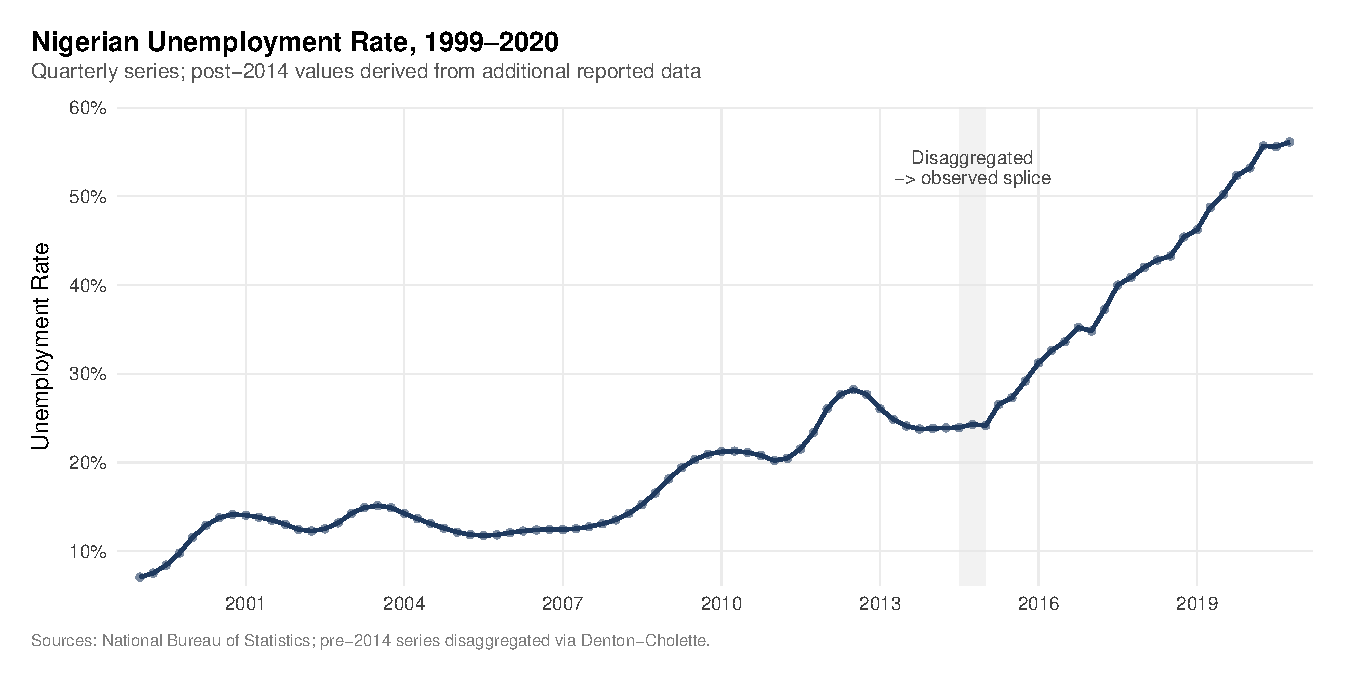
\includegraphics[keepaspectratio]{Diss_report_files/figure-pdf/fig-target-1.pdf}}

}

\caption{\label{fig-target}Quarterly unemployment rate under the 40-hour
definition, 1999 Q1 to 2020 Q4.}

\end{figure}%

Note: Pre-2014 values were temporally disaggregated from annual data
using the Denton-Cholette procedure; from 2014 Q4 onward the values are
computed from quarterly NLFS microdata. The shaded band marks the splice
point.

Figure~\ref{fig-target} shows a harmonized quarterly unemployment series
for Nigeria between 1999 and 2020 constructed under a consistent
less-than-40-hours-per-week definition of unemployment. To ensure
comparability over time, observations collected under subsequent NBS
methodologies (the 20-hour definition) were converted and temporally
disaggregated to produce a unified series. The resulting estimates
indicate a long-run increase in unemployment rate, with unemployment
rising from below 10\% in the late 1990s to over 50\% by 2020. While the
series exhibits periods of relative stability, particularly during the
early and mid-2000s, unemployment increases substantially after 2015,
reflecting the combined effects of economic slowdown, the 2016
recession, and broader structural labour market challenges. Unlike the
ILO modelled unemployment series Figure~\ref{fig-ilo-target}, which
remains below 6\% throughout the same period, this harmonized measure
captures the prevalence of insufficient labour market engagement under a
substantially stricter employment threshold. The divergence between the
two series illustrates how alternative definitions of employment can
generate markedly different assessments of labour market conditions

\begin{figure}

\centering{

\pandocbounded{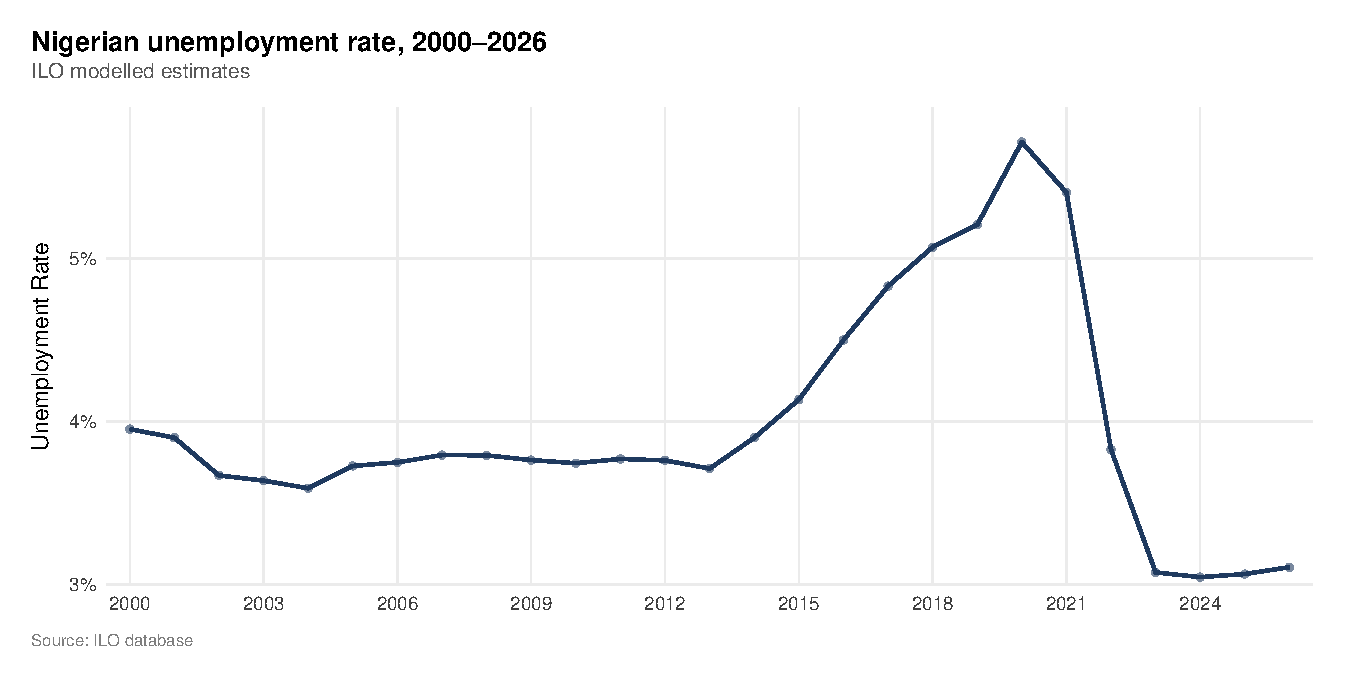
\includegraphics[keepaspectratio]{Diss_report_files/figure-pdf/fig-ilo-target-1.pdf}}

}

\caption{\label{fig-ilo-target}Yearly modelled unemployment rate under
the ILO definition}

\end{figure}%

Figure~\ref{fig-ilo-target} presents the ILO modelled unemployment rate
for Nigeria between 2000 and 2026. Unlike Nigeria's former domestic
unemployment measure, these estimates are produced using the ILO's
internationally harmonized labour force framework, which classifies
individuals as employed if they perform at least one hour of work for
pay or profit during the reference period. As a result, the series
remains consistently low, ranging from approximately 3.1\% to 5.7\% over
the period. The sharp contrast between these estimates and Nigeria's
former domestic unemployment rates highlights the extent to which
measured labour market conditions depend on the underlying definition of
employment.

\subsubsection{Spurious Correlation Arising From Common Temporal
Trends}\label{spurious-correlation-arising-from-common-temporal-trends}

\begin{figure}

\centering{

\pandocbounded{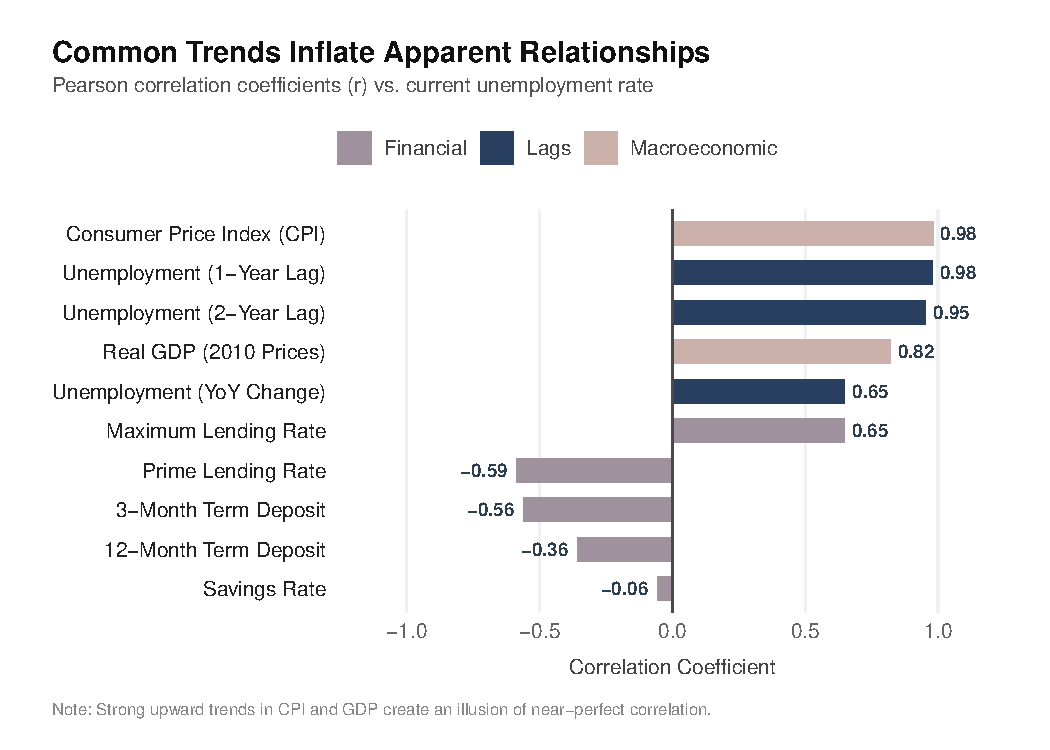
\includegraphics[keepaspectratio]{Diss_report_files/figure-pdf/fig-raw-correlation-1.pdf}}

}

\caption{\label{fig-raw-correlation}Raw Correlations of Features}

\end{figure}%

Figure~\ref{fig-raw-correlation} reports pairwise correlations between
unemployment and the candidate predictor variables using the original
non-stationary series. Several variables exhibit remarkably strong
correlations with unemployment. For example, CPI, GDP, and
autoregressive features show correlations exceeding 0.8 in absolute
value.

However, these relationships need to be carefully considered. Many
macroeconomic variables exhibit strong time trends and persistence. When
two unrelated variables trend upward over time, they may appear highly
correlated even in the absence of a meaningful economic relationship.
This phenomenon, commonly referred to as spurious correlation, creates
temporal confounding in predictive modelling.

To distinguish genuine economic relationships from common temporal
trends, I transformed the variables to achieve stationarity and the
correlation analysis is repeated below. Following differencing, several
previously strong relationships weakened substantially, while others
remained relatively robust.

\begin{figure}[H]

{\centering \pandocbounded{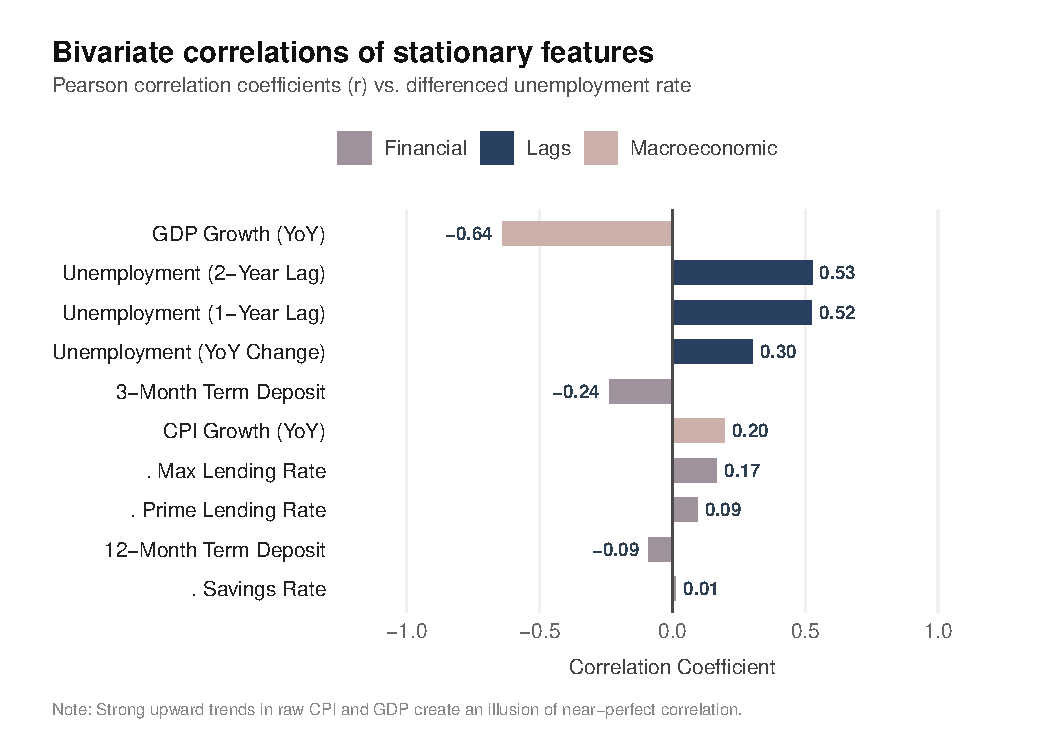
\includegraphics[keepaspectratio]{Diss_report_files/figure-pdf/Fig-stationary-correlation-1.pdf}}

}

\caption{Stationary Correlations of Features}

\end{figure}%

The comparison shows that much of the predictive power in the raw data
reflects shared temporal dynamics rather than genuine economic
relationships, so reconstruction models built on raw values risk
producing spurious results. Nevertheless, a subset of variables
continues to exhibit meaningful associations with unemployment after
stationarity adjustments, suggesting that these indicators contain
information beyond simple co-trending behaviour.

\subsection{Model evaluation}\label{model-evaluation}

\subsubsection{Elastic Net Model
Performance}\label{elastic-net-model-performance}

The Elastic Net model was evaluated using rolling-origin
cross-validation with an expanding training window.

Table~\ref{tbl-model-performance} presents the forecasting performance
metrics.

{

\begin{longtable}[]{@{}lr@{}}

\caption{\label{tbl-model-performance}Model Performance Summary}

\tabularnewline

\toprule\noalign{}
Metric & value \\
\midrule\noalign{}
\endhead
\bottomrule\noalign{}
\endlastfoot
RMSE & 2.765 \\
MAE & 2.280 \\
NRMSE & 0.080 \\
90\% Prediction Interval Coverage & 0.800 \\

\end{longtable}

}

The model achieved an RMSE of 2.765 and an MAE of 2.28, indicating that
forecasts were generally close to observed unemployment rates. The
normalized RMSE of 0.08 indicates that the forecast errors amounted to
approximately 8.05\% of the average unemployment rate, suggesting
relatively low error relative to the scale of the series.

The prediction intervals achieved a coverage rate of 80\%, compared with
the nominal 90\% level. Although slightly below the target, this
indicates that the uncertainty estimates were reasonably well
calibrated.

\subsubsection{Out-of-Sample Reconstruction
Visualization}\label{out-of-sample-reconstruction-visualization}

Figure~\ref{fig-reconstruction-visualization} compares observed and
predicted unemployment rates across the evaluation period.

The forecasts closely tracked medium-term movements in unemployment,
although some deviations occurred during periods of rapid change. This
pattern is expected because Elastic Net regression primarily captures
systematic relationships rather than unexpected shocks.

\begin{figure}[H]

\centering{

\pandocbounded{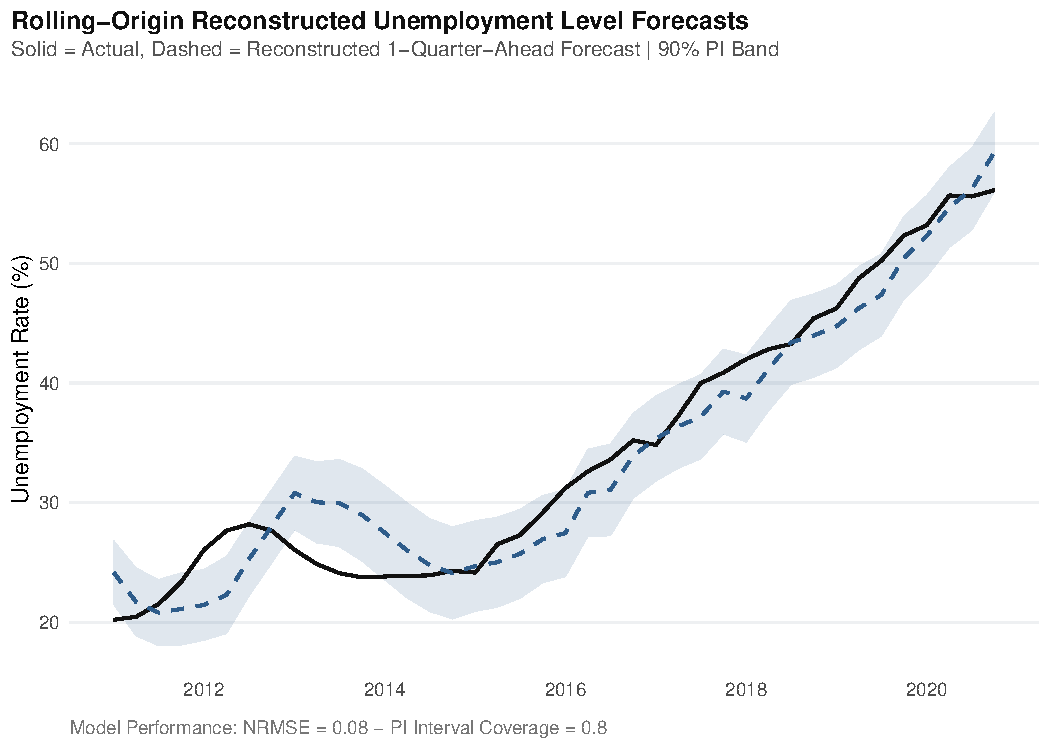
\includegraphics[keepaspectratio]{Diss_report_files/figure-pdf/fig-reconstruction-visualization-1.pdf}}

}

\caption{\label{fig-reconstruction-visualization}Rolling Out-of-Sample
Reconstruction}

\end{figure}%

\subsubsection{Digital Trace Extension}\label{digital-trace-extension}

\paragraph{Effect of Including Digital Trace
Features}\label{effect-of-including-digital-trace-features}

To assess whether digital trace data improved predictive performance,
the model was re-estimated including Google Trends search volumes which
where reduced to 2 principal components alongside the macroeconomic
predictors.

{

\begin{longtable}[]{@{}
  >{\raggedright\arraybackslash}p{(\linewidth - 8\tabcolsep) * \real{0.3289}}
  >{\raggedleft\arraybackslash}p{(\linewidth - 8\tabcolsep) * \real{0.0789}}
  >{\raggedleft\arraybackslash}p{(\linewidth - 8\tabcolsep) * \real{0.0789}}
  >{\raggedleft\arraybackslash}p{(\linewidth - 8\tabcolsep) * \real{0.0789}}
  >{\raggedleft\arraybackslash}p{(\linewidth - 8\tabcolsep) * \real{0.4342}}@{}}

\caption{\label{tbl-gt_Feature_Matrix}Extended Model Performance
Summary}

\tabularnewline

\toprule\noalign{}
\begin{minipage}[b]{\linewidth}\raggedright
Model
\end{minipage} & \begin{minipage}[b]{\linewidth}\raggedleft
RMSE
\end{minipage} & \begin{minipage}[b]{\linewidth}\raggedleft
MAE
\end{minipage} & \begin{minipage}[b]{\linewidth}\raggedleft
NRMSE
\end{minipage} & \begin{minipage}[b]{\linewidth}\raggedleft
90\% Prediction Interval Coverage
\end{minipage} \\
\midrule\noalign{}
\endhead
\bottomrule\noalign{}
\endlastfoot
Full Elastic Net & 2.765 & 2.280 & 0.080 & 0.800 \\
Full Elastic Net + Trace & 2.276 & 1.773 & 0.059 & 0.821 \\

\end{longtable}

}

The resulting model exhibited a modest improvement in predictive
accuracy relative to the macroeconomic-only specification. However, this
apparent improvement cannot be directly compared.

Unlike the benchmark model, the digital trace specification could only
be estimated using data from 2004 onwards because Google Trends data
only became available after 2004. Consequently, the inclusion of search
data substantially reduced the length of the estimation and evaluation
sample, producing a considerably shorter evaluation window which is
arguably easier to estimate. Forecasting performance is therefore not
directly comparable across the two specifications, as prediction
difficulty generally depends on the length and historical coverage of
the evaluation period.

The final forward projection reconstruction is based solely on the
macroeconomic specification, allowing for a substantially longer
estimation period while still delivering strong predictive accuracy.

\subsubsection{Comparison with Lag-Only
Model}\label{comparison-with-lag-only-model}

A naive forecast or reconstruction exercise will be based only on the
immediate past values so that serves as a good bechmark to compare our
model.

Table~\ref{tbl-model-comparison} compares forecasting accuracy.

{

\begin{longtable}[]{@{}
  >{\raggedright\arraybackslash}p{(\linewidth - 8\tabcolsep) * \real{0.3289}}
  >{\raggedleft\arraybackslash}p{(\linewidth - 8\tabcolsep) * \real{0.0789}}
  >{\raggedleft\arraybackslash}p{(\linewidth - 8\tabcolsep) * \real{0.0789}}
  >{\raggedleft\arraybackslash}p{(\linewidth - 8\tabcolsep) * \real{0.0789}}
  >{\raggedleft\arraybackslash}p{(\linewidth - 8\tabcolsep) * \real{0.4342}}@{}}

\caption{\label{tbl-model-comparison}Model Comparison Summary}

\tabularnewline

\toprule\noalign{}
\begin{minipage}[b]{\linewidth}\raggedright
Model
\end{minipage} & \begin{minipage}[b]{\linewidth}\raggedleft
RMSE
\end{minipage} & \begin{minipage}[b]{\linewidth}\raggedleft
MAE
\end{minipage} & \begin{minipage}[b]{\linewidth}\raggedleft
NRMSE
\end{minipage} & \begin{minipage}[b]{\linewidth}\raggedleft
90\% Prediction Interval Coverage
\end{minipage} \\
\midrule\noalign{}
\endhead
\bottomrule\noalign{}
\endlastfoot
Lag Only & 3.366 & 2.759 & 1.024 & 0.739 \\
Full Elastic Net & 2.765 & 2.280 & 0.080 & 0.800 \\
Full Elastic Net + Trace & 2.276 & 1.773 & 0.059 & 0.821 \\

\end{longtable}

}

As expected the model using only the one year and 2 year autoregressive
features performs worse than the models with additional information.

\subsection{Feature Importance
Analysis}\label{feature-importance-analysis}

\subsubsection{Determinants of the Domestic
Definition}\label{determinants-of-the-domestic-definition}

The coefficients of the model was used to identify the variables that
contributed most to forecasting performance.

Figure~\ref{fig-ft-importance} presents the relative importance of
retained predictors of the domestic definition excluding the most
dominant feature - GDP growth, to allow for better scaling of other
features.

The bars are coloured according to coefficient sign, indicating whether
increases in the predictor are associated with increases (positive) or
decreases (negative) in predicted unemployment.

\begin{figure}

\centering{

\pandocbounded{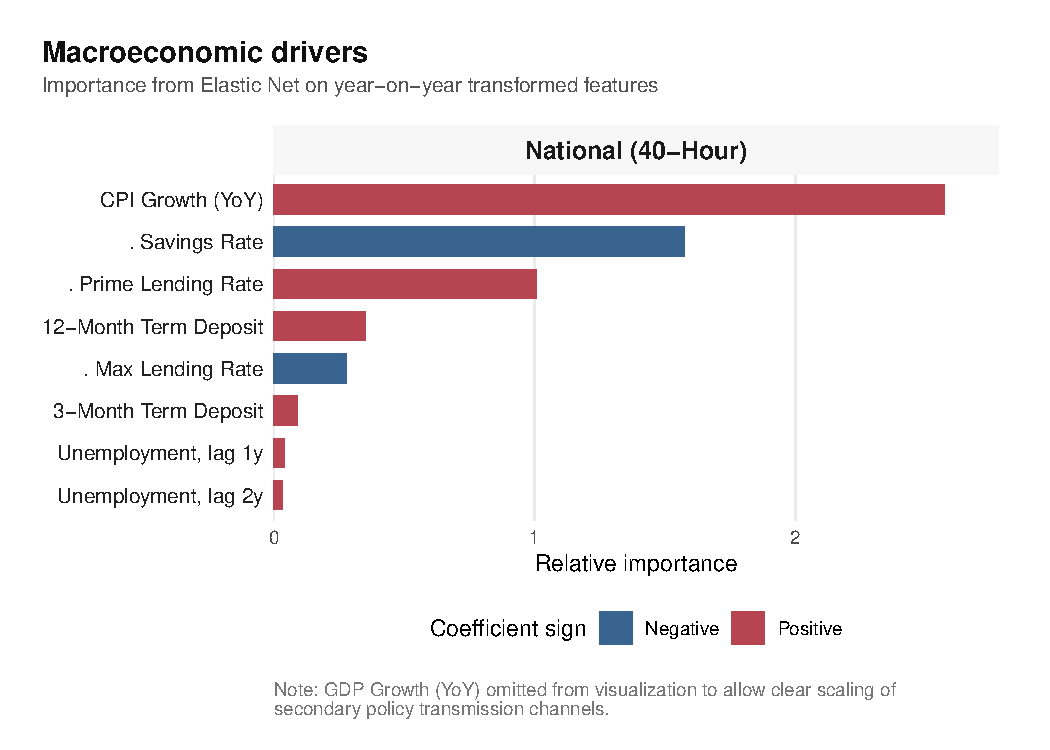
\includegraphics[keepaspectratio]{Diss_report_files/figure-pdf/fig-ft-importance-1.pdf}}

}

\caption{\label{fig-ft-importance}Feature Importances Using the Domestic
Definition}

\end{figure}%

Figure~\ref{fig-ft-importance} presents the relative importance of the
retained predictors for the domestic unemployment definition.

The domestic model suggests that, after GDP growth, inflation and
savings behaviour are the most important macroeconomic predictors of
unemployment. The domestic model places considerable importance on
inflation alongside savings rates and lending conditions, suggesting
that the historical unemployment definition was closely associated with
broader macroeconomic conditions beyond changes in output alone. This is
consistent with the conceptual basis of the 40-hour definition, which
classified individuals working fewer than 40 hours per week as
unemployed. Because this measure was intended to capture inadequate
labour utilisation rather than complete exclusion from work, it is
plausible that it responded more strongly to macroeconomic conditions
that affect the availability and intensity of work. Financial variables,
including savings and lending rates, therefore provide additional
predictive information beyond GDP growth. In contrast, the relatively
low importance of the autoregressive terms indicates that, once these
macroeconomic conditions are accounted for, historical unemployment
contributes comparatively little additional information to forecasting
performance.

\subsubsection{Determinants of the ILO
Definition}\label{determinants-of-the-ilo-definition}

\begin{figure}

\centering{

\pandocbounded{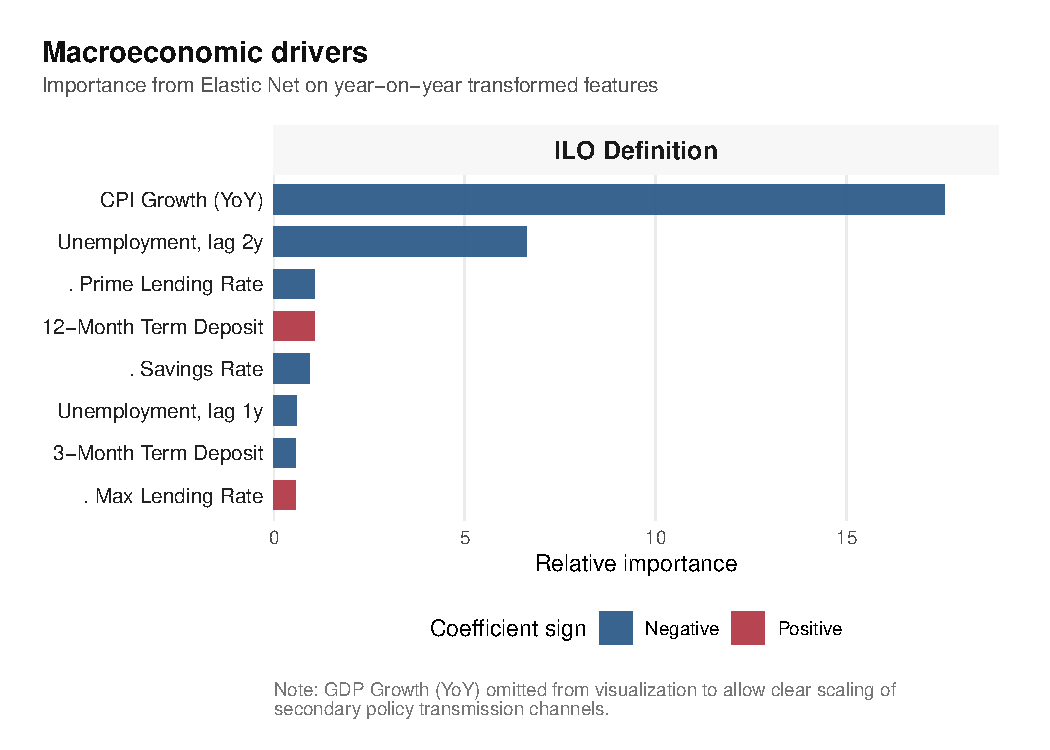
\includegraphics[keepaspectratio]{Diss_report_files/figure-pdf/fig-ft_importance-ilo-1.pdf}}

}

\caption{\label{fig-ft_importance-ilo}Feature Importance Using ILO
Definition}

\end{figure}%

Figure~\ref{fig-ft_importance-ilo} presents the relative importance of
the retained predictors for the ILO unemployment definition. As with the
domestic model, GDP growth is omitted from the visualization because it
dominated the importance rankings, allowing clearer comparison of the
remaining predictors.

Unlike the domestic definition, the ILO model is overwhelmingly
dominated by inflation, with the remaining variables contributing
substantially less predictive information. Among the retained
predictors, the two-year unemployment lag is the second most important
variable, indicating greater persistence in the ILO unemployment series.
Monetary variables, including lending rates and savings rates, remain
informative but play a comparatively smaller role. This pattern is
consistent with the conceptual basis of the ILO framework, which defines
employment using a one-hour threshold and therefore primarily captures
transitions into and out of employment rather than changes in work
intensity. Consequently, the ILO measure appears to evolve more
gradually over time and is less sensitive to broader macroeconomic
fluctuations than the historical domestic definition.

\subsubsection{Comparative Feature
Importance}\label{comparative-feature-importance}

Table~\ref{tbl-ft_importance-comp} compares the macroeconomic predictors
retained by the Elastic Net models under the historical Nigerian and ILO
unemployment definitions. Because Elastic Net performs variable
selection through coefficient shrinkage, only variables with non-zero
coefficients at the optimal penalty parameter are retained. Variables
whose coefficients were shrunk to zero were excluded, indicating that
they provided little additional predictive information after accounting
for the remaining predictors.

{

\begin{longtable}[]{@{}lll@{}}

\caption{\label{tbl-ft_importance-comp}Comparative Feature Importance of
Definitions}

\tabularnewline

\toprule\noalign{}
Variable & Domestic Rank & ILO Rank \\
\midrule\noalign{}
\endhead
\bottomrule\noalign{}
\endlastfoot
GDP Growth Rate (YoY) & 1 (Negative) & 1 (Negative) \\
Inflation Rate (CPI YoY) & 2 (Positive) & 2 (Negative) \\
Δ Savings Rate & 3 (Negative) & 6 (Negative) \\
Δ Prime Lending Rate & 4 (Positive) & 4 (Negative) \\
12-Month Term Deposit Rate (Level) & 5 (Positive) & 5 (Positive) \\
Δ Maximum Lending Rate & 6 (Negative) & 9 (Positive) \\
3-Month Term Deposit Rate (Level) & 7 (Positive) & 8 (Negative) \\
Autoregressive Lag (t-4, 1-Year) & 8 (Positive) & 7 (Negative) \\
Autoregressive Lag (t-8, 2-Year) & 9 (Positive) & 3 (Negative) \\

\end{longtable}

}

GDP growth is the dominant predictor under both unemployment
definitions, but the remaining feature rankings show clear structural
differences. Under the domestic definition, inflation and monetary
variables---including savings and lending rates---play a stronger
predictive role. The ILO model relies more heavily on lagged
unemployment, especially the two‑year term, indicating greater
persistence.

These contrasts reflect the definitions themselves. Nigeria's historical
measure classifies individuals working fewer than 40 hours per week as
unemployed, making it sensitive to reductions in work intensity. The ILO
standard counts anyone performing at least one hour of economic activity
as employed, so declines in hours or earnings that do not eliminate work
entirely affect the domestic measure more strongly. In Nigeria's
informal labour market, where workers rarely exit economic activity,
adverse conditions typically push individuals into lower‑quality or
lower‑hour jobs rather than full unemployment. The stronger role of
inflation and financial variables under the domestic definition
therefore aligns with a measure designed to capture inadequate labour
utilisation rather than outright joblessness.

Coefficient signs reinforce these differences. Inflation increases
unemployment under the ILO definition but reduces it under the domestic
measure. In Nigeria, inflation---often driven by supply‑side
pressures---tends to push households into informal or survival‑oriented
work, raising the likelihood of meeting the ILO's one‑hour threshold
while still falling short of adequate employment. Lending rates show a
similar reversal: tighter credit raises unemployment under the domestic
definition but reduces it under the ILO measure, likely reflecting
movement into informal self‑employment when formal credit access
deteriorates. These sign differences demonstrate that statistical
definitions shape observed macroeconomic relationships.

These findings should be interpreted as predictive rather than causal.
Feature importance reflects variables that improve out‑of‑sample
forecasting, and coefficient signs indicate fitted relationships.
Overall, the Domestic (40‑hour) and ILO (1‑hour) series respond
differently to identical macroeconomic conditions and cannot be treated
as interchangeable indicators of labour market distress.

\subsubsection{Feature Importance in a developed
economy}\label{feature-importance-in-a-developed-economy}

To further explore whether the macroeconomic determinants of the ILO
unemployment definition differ between developed and developing
economies, the a similar set of macroeconomic predictors was used to
model the United Kingdom's harmonised unemployment series. The United
Kingdom was selected as a developed-economy benchmark to provide a
direct comparison with the Nigerian ILO model.

{

\begin{longtable}[]{@{}
  >{\centering\arraybackslash}p{(\linewidth - 8\tabcolsep) * \real{0.0833}}
  >{\raggedright\arraybackslash}p{(\linewidth - 8\tabcolsep) * \real{0.3889}}
  >{\raggedleft\arraybackslash}p{(\linewidth - 8\tabcolsep) * \real{0.1667}}
  >{\raggedleft\arraybackslash}p{(\linewidth - 8\tabcolsep) * \real{0.2222}}
  >{\centering\arraybackslash}p{(\linewidth - 8\tabcolsep) * \real{0.1389}}@{}}

\caption{\label{tbl-Comparison_wt_Developed_Economy}UK Harmonised
Unemployment: Elastic Net feature importance and coefficient direction.}

\tabularnewline

\toprule\noalign{}
\begin{minipage}[b]{\linewidth}\centering
Rank
\end{minipage} & \begin{minipage}[b]{\linewidth}\raggedright
Variable
\end{minipage} & \begin{minipage}[b]{\linewidth}\raggedleft
Coefficient
\end{minipage} & \begin{minipage}[b]{\linewidth}\raggedleft
Rel. Importance
\end{minipage} & \begin{minipage}[b]{\linewidth}\centering
Sign
\end{minipage} \\
\midrule\noalign{}
\endhead
\bottomrule\noalign{}
\endlastfoot
1 & Inflation (CPI YoY) & 15.3902 & 100.0 & Positive \\
2 & GDP Growth (YoY) & -6.0264 & 39.2 & Negative \\
3 & Unemployment Momentum (YoY) & 0.2142 & 1.4 & Positive \\
4 & Δ Short Rate & -0.1333 & 0.9 & Negative \\
5 & AR Lag (2-year) & -0.1027 & 0.7 & Negative \\
6 & Δ Policy Rate & -0.0832 & 0.5 & Negative \\
7 & Δ Long Rate & -0.0787 & 0.5 & Negative \\
8 & AR Lag (1-year) & -0.0705 & 0.5 & Negative \\

\end{longtable}

}

Table~\ref{tbl-Comparison_wt_Developed_Economy} presents the variables
retained by the Elastic Net model for the United Kingdom's harmonised
unemployment series. Inflation (CPI year-on-year growth) emerged as the
dominant predictor, contributing substantially more to forecasting
performance than any other variable. GDP growth ranked second with a
negative coefficient, consistent with the expectation that stronger
economic growth is associated with lower unemployment. The remaining
predictors, including unemployment momentum, interest rate changes, and
autoregressive lags, contributed relatively little additional predictive
information after accounting for inflation and output growth. The
predominance of inflation is consistent with labour markets in advanced
economies, where price pressures are more closely linked to labour
market tightness and aggregate demand. Unlike the Nigerian models,
persistence plays a comparatively minor role, suggesting that current
macroeconomic conditions explain a larger share of short-term movements
in the UK's harmonised unemployment rate.

\subsection{Reconstruction of the Discontinued
Series}\label{reconstruction-of-the-discontinued-series}

The fitted model is now used to project forward the discontinued series;

\begin{figure}[H]

{\centering \pandocbounded{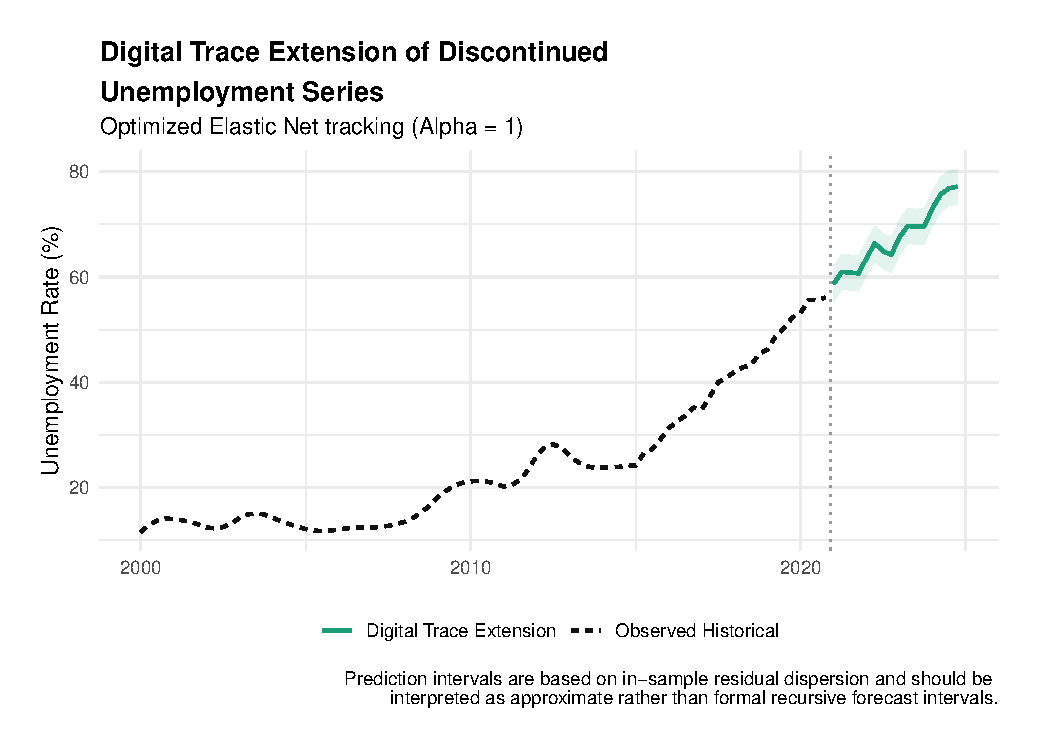
\includegraphics[keepaspectratio]{Diss_report_files/figure-pdf/Fig-reconstruction-1.pdf}}

}

\caption{Forward Projection of Discontinued Series}

\end{figure}%

The reconstructed series can be interpreted as a counterfactual
continuation of Nigeria's historical unemployment framework. Rather than
estimating a hypothetical labour market outcome, the reconstruction
seeks to answer a specific measurement question: what would reported
unemployment have looked like had the historical 40-hour definition
remained in use after 2020?

The reconstructed series suggests that considerably higher levels of
labour market distress would have been recorded under the previous
framework, as expected. Due to limitations in the
reconstruction---specifically the use of the initial 40‑hour definition
rather than the more current 20‑hour one---the series is projected to
rise as high as 77\% when forward‑projected, which may appear out of
place initially. However, considering that the Nigerian Bureau of
Statistics reported informal employment among Nigerians at 92.6\% in the
first quarter of 2023, and that this rate has consistently remained
significantly high, the projection becomes plausible.

Importantly, this does not imply that either measure is inherently
incorrect. Rather, each measure reflects a different conceptualization
of meaningful economic participation. The historical Nigerian framework
emphasized adequate labour engagement through a higher work-hour
threshold, whereas the ILO framework prioritizes international
comparability through a broader definition of employment. The
reconstruction therefore illustrates the practical consequences of
adopting one measurement philosophy over another.

\section{Discussion}\label{discussion}

\subsection{Can the Discontinued Series Be Reliably
Reconstructed?}\label{can-the-discontinued-series-be-reliably-reconstructed}

The results demonstrate that the discontinued unemployment series can be
reconstructed with a reasonable degree of accuracy using macroeconomic
indicators and autoregressive dynamics. Across the evaluation period,
the Elastic Net model consistently outperformed the lag-only benchmark,
indicating that macroeconomic conditions contain information beyond the
persistence typically observed in unemployment series. This suggests
that reconstruction is feasible and that discontinued official
statistics need not necessarily create a permanent break in longitudinal
labour market analysis.

However, the findings also illustrate the limitations of historical
reconstruction. The recursive forecasting procedure relies on its own
previous predictions, meaning that any prediction error propagates
through subsequent forecasts. Although the reconstructed trajectory
remains economically plausible over the evaluation period, forecast
uncertainty inevitably increases as the prediction horizon extends. In
practice, this implies that reconstruction is most reliable over
relatively short-to-medium horizons unless the model is periodically
recalibrated using newly observed unemployment data.

This limitation is particularly important in the context of the Nigerian
unemployment series. Because the historical 40-hour definition has been
permanently discontinued, there are no future observations against which
reconstructed values can be validated. Unlike conventional forecasting
problems, there is no opportunity to update the model or assess whether
structural changes in the economy have altered the underlying
relationship between macroeconomic variables and unemployment.
Consequently, the reconstructed series should be interpreted as a
statistically informed counterfactual rather than a replacement for
future official statistics. Its primary value lies in preserving
historical continuity and supporting longitudinal analysis, rather than
providing definitive estimates of future unemployment under the
discontinued definition.

\subsection{What Do Digital Trace Data
Contribute?}\label{what-do-digital-trace-data-contribute}

The inclusion of Google Trends variables produced a modest improvement
in predictive performance, suggesting that behavioural search activity
contains additional information relevant to labour market conditions.
This finding is broadly consistent with the digital nowcasting
literature, which argues that individuals experiencing labour market
distress often alter their online behaviour before these changes become
visible in official statistics.

However, the practical value of these gains must be interpreted in light
of an important methodological trade-off. Because Google Trends data are
only available from 2004 onwards, incorporating digital trace variables
substantially shortened both the estimation period and the out-of-sample
evaluation window. As a result, the predictive performance of the
digital trace models is not directly comparable with the benchmark
specification, since forecasting over a shorter and more recent period
is generally less challenging than reconstructing a longer historical
series spanning multiple economic regimes.

Where the objective is the historical reconstruction of discontinued
official statistics, maximizing temporal coverage may be more valuable
than obtaining marginal improvements in predictive accuracy. The
exclusion of digital trace variables from the final reconstruction model
was a methodological choice to use a model with a more extensive
evaluation window.

\subsection{What Do Different Unemployment Definitions
Measure?}\label{what-do-different-unemployment-definitions-measure}

One of the most important findings of this study is that the historical
Nigerian unemployment measure and the ILO unemployment measure capture
different dimensions of labour market performance. As shown in
Table~\ref{tbl-ft_importance-comp}, although GDP growth emerged as the
dominant predictor under both definitions, the remaining feature
rankings differ substantially. The historical domestic definition places
greater emphasis on inflation and monetary variables, whereas the ILO
definition relies more heavily on lagged unemployment, particularly the
two-year autoregressive term, indicating greater temporal persistence.
These differences suggest that changing the statistical definition
alters not only the reported unemployment rate but also the
macroeconomic relationships underlying the measure.

This divergence is consistent with the conceptual basis of the two
definitions. The historical Nigerian framework classified individuals
working fewer than 40 hours per week as unemployed, making it sensitive
to changes in work intensity and employment adequacy. By contrast, the
ILO framework classifies anyone performing at least one hour of work for
pay or profit as employed, irrespective of whether that work provides
sufficient income or stable employment. In an economy dominated by
informal and necessity-driven work, adverse macroeconomic conditions are
therefore more likely to reduce hours worked or earnings than to remove
individuals from economic activity altogether. Consequently, the
historical measure appears to capture broader labour underutilisation,
while the ILO definition primarily reflects complete labour market
exclusion.

To examine whether these relationships are specific to Nigeria (or other
developing economies) or characteristic of the ILO definition more
generally, the same modelling framework was applied to the United
Kingdom's harmonised unemployment series.
Table~\ref{tbl-Comparison_wt_Developed_Economy} shows that, while GDP
growth remained negatively associated with unemployment, inflation
overwhelmingly dominated predictive performance, contributing more than
twice the importance of GDP growth. By comparison, inflation played a
comparatively modest role under both Nigerian definitions
(Table~\ref{tbl-ft_importance-comp}). Furthermore, the Nigerian ILO
model exhibited substantially stronger dependence on lagged unemployment
than its UK counterpart, while several monetary variables changed both
their relative importance and coefficient direction across countries.

These findings suggest that adopting a common statistical definition
does not necessarily produce economically comparable unemployment
measures. Although Nigeria and the United Kingdom both report
unemployment using the internationally harmonised ILO framework,
Table~\ref{tbl-ft_importance-comp} and
Table~\ref{tbl-Comparison_wt_Developed_Economy} demonstrate that the
macroeconomic relationships underlying the measure remain strongly
influenced by the structure of each country's labour market. In advanced
economies, where unemployment primarily reflects movements into and out
of formal wage employment, inflation and business cycle conditions play
a more prominent role. In contrast, Nigeria's large informal sector
means that economic shocks are more likely to affect employment quality
and work intensity than complete labour market participation.
Consequently, statistical harmonisation improves definitional
consistency but does not necessarily harmonise the underlying economic
phenomenon being measured.

Taken together, these results reinforce the argument that unemployment
statistics are not purely objective measures but operational constructs
shaped by statistical definitions and labour market institutions.
Nigeria's transition to the ILO framework therefore represents more than
a methodological change; it changes the aspect of labour market distress
being quantified and, by extension, the macroeconomic relationships that
researchers and policymakers observe.

\subsection{Limitations}\label{limitations}

This study should be interpreted in light of several limitations
relating to both the underlying data and the reconstruction methodology.

First, the reconstructed series represents a continuation of a
historical statistical definition rather than a direct measure of
contemporary unemployment. Although the study reconstructs a consistent
40-hour unemployment series, the National Bureau of Statistics (NBS)
revised its domestic methodology in 2014 after determining that the
previous threshold no longer adequately reflected the realities of
Nigeria's evolving labour market. The revised framework lowered the
unemployment threshold to 20 hours per week and introduced a distinct
underemployment category for individuals working between 20 and 39
hours. Consequently, the post-2014 40-hour series used in this study is
not directly observed but derived from the published unemployment and
underemployment statistics to preserve consistency with the historical
definition. While this harmonization enables longitudinal
reconstruction, it implicitly assumes that the historical 40-hour
threshold remained an appropriate benchmark after 2014, an assumption
that may not fully reflect subsequent structural changes in the Nigerian
economy.

Second, the modelling framework assumes that the historical relationship
between unemployment and the selected macroeconomic indicators remains
sufficiently stable over time. Although the model demonstrated good
predictive performance during the validation period, this assumption may
weaken as the economy evolves. Structural changes in labour market
institutions, monetary policy, or employment composition could alter
these relationships, leading to forecast drift. Under normal
circumstances, such models would be periodically recalibrated using
newly observed unemployment data. However, because the historical
unemployment definition has been permanently discontinued, no future
observations exist against which the reconstructed series can be
validated or the model updated.

Finally, the study is constrained by the availability of explanatory
variables. The analysis relies primarily on aggregate macroeconomic
indicators, which cannot fully capture regional, sectoral, or
demographic heterogeneity in labour market conditions. Although
behavioural digital trace data produced modest improvements in
predictive performance, their inclusion substantially shortened the
estimation period because Google Trends data are only available from
2004 onwards. Given the study's objective of reconstructing the longest
possible historical series, preserving temporal coverage was prioritised
over marginal improvements in predictive accuracy.

These limitations suggest that the reconstructed series should be
interpreted as a statistically informed counterfactual that preserves
historical continuity rather than a definitive estimate of the
unemployment rate that would have been officially reported.
Nevertheless, the framework provides a transparent and empirically
validated approach for recovering discontinued statistical series,
particularly in settings where methodological changes interrupt
long-term economic analysis.

\clearpage

\section{References}\label{references}

\protect\phantomsection\label{refs}
\begin{CSLReferences}{1}{1}
\bibitem[\citeproctext]{ref-a2011}
A, Sodipe, Ogunrinola, and Isaiah Olurinola. 2011. {``Employment and
{Economic Growth Nexus} in {Nigeria}.''} \emph{International Journal of
Business and Social Science} 2 (January): 232--39.

\bibitem[\citeproctext]{ref-abiodun2025}
Abiodun, Adekoya, Magaji Sule, and Yahaya Ismail. 2025. \emph{Empirical
{Analysis Of The Impact Of Unemployment On Economic Growth In Nigeria}}.
13 (May): 63--80. \url{https://doi.org/10.5281/zenodo.15311427}.

\bibitem[\citeproctext]{ref-adu2023}
Adu, Williams Kwasi, Peter Appiahene, and Stephen Afrifa. 2023.
{``{VAR}, {ARIMAX} and {ARIMA} Models for Nowcasting Unemployment Rate
in {Ghana} Using {Google} Trends.''} \emph{Journal of Electrical Systems
and Information Technology} 10 (1): 12.
\url{https://doi.org/10.1186/s43067-023-00078-1}.

\bibitem[\citeproctext]{ref-alenda-demoutiez2020}
Alenda-Demoutiez, Juliette, and Daniel Mügge. 2020. {``The {Lure} of
{Ill-Fitting Unemployment Statistics}: {How South Africa}'s {Discouraged
Work Seekers Disappeared From} the {Unemployment Rate}.''} \emph{New
Political Economy} 25 (4): 590--606.
\url{https://doi.org/10.1080/13563467.2019.1613355}.

\bibitem[\citeproctext]{ref-aro2023}
Aro, Busola. 2023. {``'{I} Resisted It for 10 Years' --- {Yemi Kale}
Faults New Methodology for Unemployment Data.''} \emph{TheCable},
August.

\bibitem[\citeproctext]{ref-askitas2015}
Askitas, Nikolaos, and Klaus F Zimmermann. 2015. \emph{The {Internet} as
a {Data Source} for {Advancement} in {Social Sciences}}.

\bibitem[\citeproctext]{ref-askitas2009}
Askitas, Nikos, and Klaus F. Zimmermann. 2009. {``Google {Econometrics}
and {Unemployment Forecasting}.''} \emph{SSRN Electronic Journal}, ahead
of print, June. \url{https://doi.org/10.2139/SSRN.1480251}.

\bibitem[\citeproctext]{ref-baah-boateng2015}
Baah-Boateng, William. 2015. {``Unemployment in {Africa}.''}
\emph{International Journal of Manpower} (Bradford, United Kingdom) 36
(5): 650--67. \url{https://doi.org/10.1108/IJM-02-2014-0047}.

\bibitem[\citeproctext]{ref-ball2019}
Ball, Laurence, Davide Furceri, Daniel Leigh, and Prakash Loungani.
2019. {``Does {One Law Fit All}? {Cross-Country Evidence} on {Okun}'s
{Law}.''} \emph{Open Economies Review} 30 (5): 841--74.
\url{https://doi.org/10.1007/s11079-019-09549-3}.

\bibitem[\citeproctext]{ref-benanav2019}
Benanav, Aaron. 2019. {``The Origins of Informality: The {ILO} at the
Limit of the Concept of Unemployment.''} \emph{Journal of Global
History} 14 (1): 107--25.
\url{https://doi.org/10.1017/S1740022818000372}.

\bibitem[\citeproctext]{ref-bergmeir2012}
Bergmeir, Christoph, and José M. Benítez. 2012. {``On the Use of
Cross-Validation for Time Series Predictor Evaluation.''}
\emph{Information Sciences}, Data {Mining} for {Software
Trustworthiness}, vol. 191 (May): 192--213.
\url{https://doi.org/10.1016/j.ins.2011.12.028}.

\bibitem[\citeproctext]{ref-brandolini2006}
Brandolini, Andrea, Piero Cipollone, and Eliana Viviano. 2006. {``Does
the {Ilo Definition Capture All Unemployment}?''} \emph{Journal of the
European Economic Association} 4 (1): 153--79.
\url{https://doi.org/10.1162/jeea.2006.4.1.153}.

\bibitem[\citeproctext]{ref-byrne2004}
Byrne, David, and Eric Strobl. 2004. {``Defining Unemployment in
Developing Countries: Evidence from {Trinidad} and {Tobago}.''}
\emph{Journal of Development Economics} 73 (1): 465--76.
\url{https://doi.org/10.1016/j.jdeveco.2002.12.005}.

\bibitem[\citeproctext]{ref-choi2009}
Choi, Hyunyoung. 2009. {``Predicting {Initial Claims} for {Unemployment
Benefits}.''} July.

\bibitem[\citeproctext]{ref-damuri}
D'Amuri, Francesco. n.d. \emph{Predicting Unemployment in Short Samples
with Internet Job Search Query Data}.

\bibitem[\citeproctext]{ref-damuri2010}
D'Amuri, Francesco, and Juri Marcucci. 2010. {``'{Google It}!'
{Forecasting} the {US Unemployment Rate} with {A Google Job Search
Index}.''} \emph{SSRN Electronic Journal}, ahead of print.
\url{https://doi.org/10.2139/ssrn.1594132}.

\bibitem[\citeproctext]{ref-kale2023}
Daily Trust. 2023. {``'{It} Doesn't Make Sense',
Ex-{Statistician-General} Faults {NBS}...''} \emph{Daily Trust}, August.

\bibitem[\citeproctext]{ref-essien}
Essien, Sunday N, Garba A Manya, Mary O A Arigo, et al. n.d.
\emph{Monetary Policy and Unemployment in {Nigeria}: {Is} There a
Dynamic Relationship?}

\bibitem[\citeproctext]{ref-gayaker2025}
Gayaker, Savaş, and Hasan Türe. 2025. {``National {Unemployment Rate
Forecast} with {Google Trends}.''} \emph{Mehmet Akif Ersoy Üniversitesi
İktisadi Ve İdari Bilimler Fakültesi Dergisi} 12 (1): 107--23.
\url{https://doi.org/10.30798/makuiibf.1446639}.

\bibitem[\citeproctext]{ref-grybauskas2023}
Grybauskas, Andrius, Vaida Pilinkienė, Mantas Lukauskas, Alina
Stundžienė, and Jurgita Bruneckienė. 2023. {``Nowcasting {Unemployment
Using Neural Networks} and {Multi-Dimensional Google Trends Data}.''}
\emph{Economies} 11 (5).
\url{https://doi.org/10.3390/economies11050130}.

\bibitem[\citeproctext]{ref-guataqui2006}
Guataquí, Juan C., and Rodrigo Taborda. 2006. {``Theoretical and
Empirical Implications of the New Definition of Unemployment in
{Colombia}.''} \emph{Revista de Economía Del Rosario} 9 (1): 21--38.

\bibitem[\citeproctext]{ref-hussmanns2007}
Hussmanns, Ralf. 2007. {``Measurement of Employment, Unemployment and
Underemployment -- {Current} International Standards and Issues in Their
Application.''} \emph{Bulletin of Labour Statistics} (Geneva,
SWITZERLAND), no. 1 (January): vii--xxxi.

\bibitem[\citeproctext]{ref-ilo2023}
International Conference of Labour Statisticians. 2023. \emph{Resolution
{II}. {Resolution} to Amend the 19th {ICLS} Resolution Concerning
Statistics of Work, Employment and Labour Underutilization}. 21st.
International Labour Organization.

\bibitem[\citeproctext]{ref-icls1982}
International Labour Organization. 1982. \emph{Resolution Concerning
Statistics of the Economically Active Population, Employment,
Unemployment and Underemployment, Adopted by the {Thirteenth
International Conference} of {Labour Statisticians} ({October} 1982)}.
No. 13th. Geneva, SWITZERLAND.

\bibitem[\citeproctext]{ref-ILO2011}
International Labour Organization. 2011. \emph{Beyond the Measurement of
Unemployment and Underemployment}.
Https://www.ilo.org/publications/beyond-measurement-unemployment-and-underemployment.

\bibitem[\citeproctext]{ref-Ilo_methodology}
International Labour Organization. 2026. \emph{{ILO} Modelled Estimates
{Methodological} Overview}.

\bibitem[\citeproctext]{ref-icls100years}
International Labour Organization. n.d. \emph{International {Conference}
of {Labour Statisticians} ({ICLS}) - {ILOSTAT}}.
Https://ilostat.ilo.org/about/standards/icls/?playlist=4194a13\&video=38313ec.

\bibitem[\citeproctext]{ref-kale2015}
Kale, Yemi, and Sani I. Doguwa. 2015. {``On the {Compilation} of {Labour
Force Statistics} for {Nigeria}.''} \emph{CBN Journal of Applied
Statistics} 6 (1(a)): 183--98.

\bibitem[\citeproctext]{ref-krishnamurthy}
Krishnamurthy, Shree Hari. n.d. \emph{A {Comprehensive} Study of
Applying Machine Learning Algorithms for Time Series Data Prediction to
the {Irish Labour Market Unemployment Rate}}.

\bibitem[\citeproctext]{ref-morse1970}
Morse, David A. 1970. {``Unemployment in {Developing Countries}.''}
\emph{Political Science Quarterly} 85 (1): 1--16.
\url{https://doi.org/10.2307/2147555}.

\bibitem[\citeproctext]{ref-mulero2023}
Mulero, Rodrigo, and Alfredo Garcia-Hiernaux. 2023. {``Forecasting
Unemployment with {Google Trends}: Age, Gender and Digital Divide.''}
\emph{Empirical Economics} 65 (2): 587--605.
\url{https://doi.org/10.1007/s00181-022-02347-w}.

\bibitem[\citeproctext]{ref-nationalbureauofstatistics2016}
National Bureau of Statistics. 2016.
\emph{{UNEMPLOYMENT}/{UNDER}-{EMPLOYMENT REPORT Q2} 2016}. Q2 2016.
National Bureau of Statistics (Nigeria).

\bibitem[\citeproctext]{ref-nationalbureauofstatistics2021}
National Bureau of Statistics. 2021. \emph{Labour {Force Statistics}:
{Unemployment} and {Underemployment Report} ({Q4} 2020)}. Q4 2020.
National Bureau of Statistics (Nigeria).

\bibitem[\citeproctext]{ref-nationalbureauofstatistics2023}
National Bureau of Statistics. 2023. \emph{Nigerian {Labour Force
Statistics Report Q4} 2022 \& {Q1} 2023}. Q4 2022 \& Q1 2023. National
Bureau of Statistics (Nigeria).

\bibitem[\citeproctext]{ref-ojapinwa2013}
Ojapinwa, Taiwo, and Esan Folorunso. 2013. {``Does {Philips Relations
Really Exist} in {Nigeria}? {Empirical Evidence}.''} \emph{International
Journal of Economics and Finance} 5 (August): 123--23.
\url{https://doi.org/10.5539/ijef.v5n9p123}.

\bibitem[\citeproctext]{ref-olukanmi2021}
Olukanmi, Seun O., Fulufhelo V. Nelwamondo, and Nnamdi I. Nwulu. 2021.
{``Utilizing {Google Search Data With Deep Learning}, {Machine Learning}
and {Time Series Modeling} to {Forecast Influenza-Like Illnesses} in
{South Africa}.''} \emph{IEEE Access} 9: 126822--36.
\url{https://doi.org/10.1109/ACCESS.2021.3110972}.

\bibitem[\citeproctext]{ref-pavlicek2015}
Pavlicek, Jaroslav, and Ladislav Kristoufek. 2015. {``Nowcasting
{Unemployment Rates} with {Google Searches}: {Evidence} from the
{Visegrad Group Countries}.''} \emph{PLOS ONE} 10 (5): e0127084.
\url{https://doi.org/10.1371/journal.pone.0127084}.

\bibitem[\citeproctext]{ref-Proshare2023}
Proshare Research. 2023. \emph{Nigeria's {New Unemployment Data} in
{Numbers}: {Reality}, {Revision}, and {Reflection} - {Proshare}}.
Https://www.proshare.co/articles/nigerias-new-unemployment-data-in-numbers-reality-revision-and-reflection?menu=Economy\&classification=Read\&category=Nigeria+Economy.

\bibitem[\citeproctext]{ref-richardson1992}
Richardson, S. C., Ralf Hussmanns, Farhad Mehran, and Vijay Verma. 1992.
{``Surveys of {Economically Active Population}, {Employment},
{Unemployment} and {Underemployment}.''} \emph{The Statistician} 41 (2):
249. \url{https://doi.org/10.2307/2348265}.

\bibitem[\citeproctext]{ref-hyndman2018}
Rob J Hyndman, and George Athanasopoulos. n.d. \emph{Forecasting:
{Principles} and {Practice} (2nd Ed)}.

\bibitem[\citeproctext]{ref-smith2016}
Smith, Paul. 2016. {``Google's {MIDAS Touch}: {Predicting UK
Unemployment} with {Internet Search Data}.''} \emph{Journal of
Forecasting} 35 (3): 263--84. \url{https://doi.org/10.1002/for.2391}.

\bibitem[\citeproctext]{ref-tule2016}
Tule, Moses, Taiwo Ajilore, and Godday Ebuh. 2016. {``A Composite Index
of Leading Indicators of Unemployment in {Nigeria}.''} \emph{Journal of
African Business} 17 (1): 87--105.
\url{https://doi.org/10.1080/15228916.2016.1113909}.

\bibitem[\citeproctext]{ref-umoru2013}
Umoru, David, and M. A. Anyiwe. 2013. {``Dynamics of {Inflation} and
{Unemployment} in a {Vector Error Correction Model}.''} \emph{Research
on Humanities and Social Sciences} 3 (3): 20.

\bibitem[\citeproctext]{ref-vera-jaramillo2025}
Vera-Jaramillo, Jaime. 2025. \emph{Reconstructing {Subnational Labor
Indicators} in {Colombia}: {An Integrated Machine} and {Deep Learning
Approach}}. arXiv:2508.12514. arXiv.
\url{https://doi.org/10.48550/arXiv.2508.12514}.

\bibitem[\citeproctext]{ref-wikipedia_minwage}
Wikipedia contributors. 2026. {``List of Countries by Minimum Wage.''}
\emph{Wikipedia}, April.

\bibitem[\citeproctext]{ref-dichotomy2023}
World Bank. n.d. {``Nigeria's Dichotomy: Low Unemployment, High Poverty
Rates.''} In \emph{World Bank Blogs}.
Https://blogs.worldbank.org/en/opendata/nigerias-dichotomy-low-unemployment-high-poverty-rates.

\bibitem[\citeproctext]{ref-yi2021}
Yi, Dingdong, Shaoyang Ning, Chia Jung Chang, and S. C. Kou. 2021.
{``Forecasting {Unemployment Using Internet Search Data} via {PRISM}.''}
\emph{Journal of the American Statistical Association} 116 (536):
1662--73. \url{https://doi.org/10.1080/01621459.2021.1883436}.

\end{CSLReferences}

\clearpage

\section{Appendix}\label{appendix}

Source code and extra materials can be found in
\href{https://github.com/olaa003/NG_unemployment_trace}{this}
reprository.

\begingroup
\setlength\LTleft{0.05\linewidth}
\setlength\LTright{0.05\linewidth}\fontsize{10.0pt}{12.0pt}\selectfont

\begin{longtable}{@{\extracolsep{\fill}}>{\raggedright\arraybackslash}p{\dimexpr 0.18\linewidth -2\tabcolsep-1.5\arrayrulewidth}>{\raggedright\arraybackslash}p{\dimexpr 0.14\linewidth -2\tabcolsep-1.5\arrayrulewidth}>{\raggedright\arraybackslash}p{\dimexpr 0.58\linewidth -2\tabcolsep-1.5\arrayrulewidth}}

\caption{\label{tbl-country_minwage}Wikipedia contributors (2026)}

\tabularnewline

\caption*{
{\fontsize{20}{25}\selectfont  Minimum wage basis by country (Abridged)\fontsize{10}{12}\selectfont }
} \\ 
\toprule
Country & Wage Basis & Notes \\ 
\midrule\addlinespace[2.5pt]
Afghanistan & {\cellcolor[HTML]{EAF3DE}{monthly}} & Afs 5500/month for non-permanent private sector \\ 
Albania & {\cellcolor[HTML]{EAF3DE}{monthly}} & L39087/month (\textasciitilde{}€471) \\ 
Algeria & {\cellcolor[HTML]{FBEAF0}{both}} & DA 24000/month; DA 138.46/hour also published \\ 
Andorra & {\cellcolor[HTML]{E6F1FB}{hourly}} & €7.70/hour \\ 
Angola & {\cellcolor[HTML]{EAF3DE}{monthly}} & Kz 32181/month paid 13x per year \\ 
Antigua \& Barbuda & {\cellcolor[HTML]{E6F1FB}{hourly}} & EC\$8.20/hour \\ 
Armenia & {\cellcolor[HTML]{EAF3DE}{monthly}} & 75000 AMD/month (\textasciitilde{}\$190) \\ 
Australia & {\cellcolor[HTML]{E6F1FB}{hourly}} & Award-based; national minimum wage set per hour \\ 
Austria & {\cellcolor[HTML]{F1EFE8}{none}} & No national minimum; collective bargaining by sector \\ 
Azerbaijan & {\cellcolor[HTML]{EAF3DE}{monthly}} & 345 AZN/month (\textasciitilde{}\$203) \\ 
Bahamas & {\cellcolor[HTML]{E6F1FB}{hourly}} & B\$5.25/hour (also daily/weekly equivalents) \\ 
Bahrain & {\cellcolor[HTML]{F1EFE8}{none}} & Public-sector floor only; no private-sector statutory minimum \\ 
Bangladesh & {\cellcolor[HTML]{EAF3DE}{monthly}} & 1500 BDT/month; industry-specific rates vary \\ 
Barbados & {\cellcolor[HTML]{E6F1FB}{hourly}} & Bds\$10.50-\$11.43/hour by category \\ 
Belarus & {\cellcolor[HTML]{EAF3DE}{monthly}} & Br 554/month (\textasciitilde{}\$122) \\ 
Belgium & {\cellcolor[HTML]{EAF3DE}{monthly}} & €2030/month \\ 
Belize & {\cellcolor[HTML]{E6F1FB}{hourly}} & BZ\$5.00/hour \\ 
Benin & {\cellcolor[HTML]{EAF3DE}{monthly}} & CFA 52000/month \\ 
Bhutan & {\cellcolor[HTML]{EAF3DE}{monthly}} & Nu 3750/month \\ 
Bolivia & {\cellcolor[HTML]{EAF3DE}{monthly}} & Bs. 2500/month + Christmas bonus \\ 
Bosnia \& Herzegovina & {\cellcolor[HTML]{EAF3DE}{monthly}} & KM 543 net/month (\textasciitilde{}\$269) \\ 
Botswana & {\cellcolor[HTML]{E6F1FB}{hourly}} & P 7.34/hour (also monthly equivalent) \\ 
Brazil & {\cellcolor[HTML]{EAF3DE}{monthly}} & R\$1621/month paid 13x per year \\ 
Brunei & {\cellcolor[HTML]{F1EFE8}{none}} & No statutory minimum wage \\ 
Bulgaria & {\cellcolor[HTML]{FBEAF0}{both}} & 1077 BGN/month and 6.49 BGN/hour both official \\ 
Burkina Faso & {\cellcolor[HTML]{EAF3DE}{monthly}} & CFA 34664/month \\ 
Cambodia & {\cellcolor[HTML]{EAF3DE}{monthly}} & KHR 818800/month (\textasciitilde{}\$200) textiles sector \\ 
Cameroon & {\cellcolor[HTML]{EAF3DE}{monthly}} & CFA 36270/month \\ 
Canada & {\cellcolor[HTML]{E6F1FB}{hourly}} & Set per province/territory; federal floor also hourly \\ 
Cape Verde & {\cellcolor[HTML]{EAF3DE}{monthly}} & 13000 CVE/month (\textasciitilde{}\$141) \\ 
Central African Republic & {\cellcolor[HTML]{FBEAF0}{both}} & FCFA 35000/month and FCFA 218.75/hour \\ 
Chad & {\cellcolor[HTML]{FBEAF0}{both}} & FCFA 59995/month and FCFA 355/hour \\ 
Chile & {\cellcolor[HTML]{EAF3DE}{monthly}} & CL\$529000/month for workers 18-65 \\ 
China & {\cellcolor[HTML]{FBEAF0}{both}} & Set locally; expressed monthly or hourly depending on region \\ 
Colombia & {\cellcolor[HTML]{EAF3DE}{monthly}} & COP 1423500 + COP 200000 transport/month \\ 
Comoros & {\cellcolor[HTML]{EAF3DE}{monthly}} & CF 55000/month \\ 
DR Congo & {\cellcolor[HTML]{FAEEDA}{daily}} & FC 1680/day (\textasciitilde{}\$1.83) \\ 
Republic of Congo & {\cellcolor[HTML]{EAF3DE}{monthly}} & FCFA 90000/month (formal sector) \\ 
Costa Rica & {\cellcolor[HTML]{FAEEDA}{daily}} & 11954-16000 CRC/day by sector \\ 
Cote d'Ivoire & {\cellcolor[HTML]{EAF3DE}{monthly}} & CFA 60000/month (lowest category) \\ 
Croatia & {\cellcolor[HTML]{EAF3DE}{monthly}} & €840/month \\ 
Cuba & {\cellcolor[HTML]{EAF3DE}{monthly}} & \$MN 2100/month (\textasciitilde{}\$6.66) \\ 
Czech Republic & {\cellcolor[HTML]{FBEAF0}{both}} & CZK 20800/month; CZK 124.40/hour \\ 
Denmark & {\cellcolor[HTML]{F1EFE8}{none}} & No statutory minimum; collective bargaining (avg \textasciitilde{}DKK 110/hr) \\ 
Djibouti & {\cellcolor[HTML]{F1EFE8}{none}} & 2006 Labour Code replaced fixed rate with sector negotiations \\ 
Dominica & {\cellcolor[HTML]{E6F1FB}{hourly}} & EC\$4.00/hour \\ 
Dominican Republic & {\cellcolor[HTML]{EAF3DE}{monthly}} & RD\$8310-\$15100/month by sector \\ 
Ecuador & {\cellcolor[HTML]{EAF3DE}{monthly}} & \$594/month (includes 13th \& 14th salary components) \\ 
Egypt & {\cellcolor[HTML]{EAF3DE}{monthly}} & Public sector: EGP 6000/month; private sector floor varies \\ 
El Salvador & {\cellcolor[HTML]{EAF3DE}{monthly}} & \$304.17/month \\ 
Equatorial Guinea & {\cellcolor[HTML]{EAF3DE}{monthly}} & FCFA 129035/month \\ 
Estonia & {\cellcolor[HTML]{FBEAF0}{both}} & €725/month; €4.30/hour \\ 
Eswatini & {\cellcolor[HTML]{EAF3DE}{monthly}} & E 420-531/month by sector \\ 
Ethiopia & {\cellcolor[HTML]{F1EFE8}{none}} & No national minimum; some state enterprises set own floors \\ 
Fiji & {\cellcolor[HTML]{E6F1FB}{hourly}} & FJ\$2.68/hour \\ 
Finland & {\cellcolor[HTML]{F1EFE8}{none}} & No statutory minimum; sector collective agreements required \\ 
France & {\cellcolor[HTML]{FBEAF0}{both}} & €1801/month (official SMIC); €11.88/hour equivalent \\ 
Gabon & {\cellcolor[HTML]{EAF3DE}{monthly}} & FCFA 150000/month \\ 
\bottomrule

\end{longtable}

\endgroup

Source: Data compiled from Wikipedia contributors (2026)

\clearpage

\begingroup
\setlength\LTleft{0\linewidth}
\setlength\LTright{0\linewidth}\fontsize{10.0pt}{12.0pt}\selectfont

\begin{longtable}{@{\extracolsep{\fill}}>{\raggedright\arraybackslash}p{\dimexpr 0.12\linewidth -2\tabcolsep-1.5\arrayrulewidth}>{\raggedleft\arraybackslash}p{\dimexpr 0.08\linewidth -2\tabcolsep-1.5\arrayrulewidth}>{\raggedright\arraybackslash}p{\dimexpr 0.80\linewidth -2\tabcolsep-1.5\arrayrulewidth}}

\caption{\label{tbl-icls-sessions}International Labour Organization
(n.d.)}

\tabularnewline

\caption*{
{\fontsize{20}{25}\selectfont  International Conference of Labour Statisticians (ICLS): Sessions and Key Resolutions\fontsize{10}{12}\selectfont }
} \\ 
\toprule
Session & Year & Key Resolutions / What Was Introduced \\ 
\midrule\addlinespace[2.5pt]
1st ICLS & 1923 & First international guidelines on labour statistics; basic definitions of employment and wages \\ 
2nd ICLS & 1925 & Standards on wages and hours of work statistics \\ 
3rd ICLS & 1926 & Guidelines on unemployment statistics; resolution on statistics of collective agreements \\ 
4th ICLS & 1931 & Standards on statistics of industrial disputes and strikes \\ 
5th ICLS & 1937 & Revised guidelines on wages and hours; led to ILC Convention No. 63 on wages and hours of work \\ 
6th ICLS & 1947 & Post-war revival; guidelines on labour force statistics and employment measurement \\ 
7th ICLS & 1949 & Standards on family living studies and household expenditure \\ 
8th ICLS & 1954 & Revised definitions of employment and unemployment; guidelines on migration statistics \\ 
9th ICLS & 1957 & Standards on statistics of occupational injuries and diseases \\ 
10th ICLS & 1962 & Guidelines on labour cost statistics; revision of wages and hours standards \\ 
11th ICLS & 1966 & Standards on measurement and analysis of underemployment and underutilization of manpower \\ 
12th ICLS & 1973 & Revised integrated system of wages statistics; household income and expenditure survey guidelines \\ 
13th ICLS & 1982 & Landmark resolution on the economically active population — modern definitions of employment, unemployment and underemployment \\ 
14th ICLS & 1987 & Guidelines on occupational injuries statistics; statistics of collective bargaining \\ 
15th ICLS & 1993 & First standards on statistics of employment in the informal sector \\ 
16th ICLS & 1998 & Resolution on measurement of employment-related income; underemployment and inadequate employment; CPI guidelines \\ 
17th ICLS & 2003 & Guidelines on informal employment (broadening 15th ICLS); CPI standards; called for ISCO-88 revision \\ 
18th ICLS & 2008 & Resolution on child labour statistics; decent work measurement guidelines; amendment to 13th ICLS resolution \\ 
19th ICLS & 2013 & Major overhaul — five forms of work; redefined employment as work for pay or profit; LU1-LU4 labour underutilization measures \\ 
20th ICLS & 2018 & Resolution on work relationships (ICSE-18); amendment to 18th ICLS child labour resolution; SDG indicator methodology \\ 
21st ICLS & 2023 & Resolution on statistics of the informal economy; amendments to 19th, 16th, and 17th ICLS resolutions \\ 
\bottomrule

\end{longtable}

\endgroup

Source: Data compiled from International Labour Organization (n.d.) and
ILO reports.

\clearpage




\end{document}
